%# -*- coding: utf-8-unix -*-
%%==================================================
%% thesis.tex
%%==================================================

% 双面打印
\documentclass[master, fontset=adobe, openright, twoside]{sjtuthesis}
% \documentclass[bachelor, fontset=adobe, openany, oneside, submit]{sjtuthesis} 
% \documentclass[master, adobefonts, review]{sjtuthesis} 
% \documentclass[%
%   bachelor|master|doctor,	% 必选项
%   fontset=adobe|windows,  	% 只测试了adobe
%   oneside|twoside,		% 单面打印,双面打印(奇偶页交换页边距,默认)
%   openany|openright, 		% 可以在奇数或者偶数页开新章|只在奇数页开新章(默认)
%   zihao=-4|5,, 		% 正文字号:小四、五号(默认)
%   review,	 		% 盲审论文,隐去作者姓名、学号、导师姓名、致谢、发表论文和参与的项目
%   submit			% 定稿提交的论文,插入签名扫描版的原创性声明、授权声明 
% ]

% 逐个导入参考文献数据库
\addbibresource{bib/thesis.bib}
% \addbibresource{bib/chap2.bib}
\usepackage{setspace}
\usepackage{comment}
\linespread{1.6}
\begin{document}

%\bibliographystyle{plain}
%% 无编号内容:中英文论文封面、授权页
%# -*- coding: utf-8-unix -*-
\title{上海交通大学学位论文 \LaTeX 模板示例文档}
\author{某某}
\advisor{某某教授}
% \coadvisor{某某教授}
\defenddate{2017年1月17日}
\school{上海交通大学}
\institute{某某系}
\studentnumber{1140329042}
\major{某某专业}

\englishtitle{A Sample Document for \LaTeX-basedd SJTU Thesis Template}
\englishauthor{\textsc{Mo Mo}}
\englishadvisor{Prof. \textsc{Mou Mou}}
% \englishcoadvisor{Prof. \textsc{Uom Uom}}
\englishschool{Shanghai Jiao Tong University}
\englishinstitute{\textsc{Depart of XXX, School of XXX} \\
  \textsc{Shanghai Jiao Tong University} \\
  \textsc{Shanghai, P.R.China}}
\englishmajor{A Very Important Major}
\englishdate{Dec. 17th, 2014}


\maketitle

\makeenglishtitle

\makeatletter
\ifsjtu@submit\relax
	\includepdf{pdf/original.pdf}
	\cleardoublepage
	\includepdf{pdf/authorization.pdf}
	\cleardoublepage
\else
	\makeDeclareOriginal
	\makeDeclareAuthorization
\fi
\makeatother


\frontmatter 	% 使用罗马数字对前言编号

%% 摘要
\pagestyle{main}
%# -*- coding: utf-8-unix -*-
%%==================================================
%% abstract.tex for SJTU Master Thesis
%%==================================================

\begin{abstract}
现如今,机器人在我们的社会生产生活当中发挥着越来越大的作用,可以帮助人们从繁重工作或者简单重复性的工作中解脱出来并且能够在高温、低压、辐射等不适宜人作业的高危环境下工作。从而极大的提高了生产效率。然而随着工作环境以及任务越来越复杂,单个机器人的能力由于成本以及结构等因素而变得有限。相比单个机器人,多机器人系统由于其系统冗余,结构多变,配置简单等特点,可以降低系统单一成本,提高系统效率和鲁棒性,因而在某些作业环境下更具优势。

在某些应用场景下,多机器人经常需要根据任务组成特定的队形,即多机器人编队技术。多机器人编队是指多个自主移动机器人在运动过程中保持某种队形的技术。这一技术被广泛应用在军事侦察、地形搜索、灾难救援、货物搬运等复杂任务。在这些工作任务中,由于机器人之间需要通信与协作,因此编队的同步性就显得尤为重要。例如在协同搬运过程中,如果机器人之间的运动不同步,则很有可能导致搬运的物体受力不均而造成损坏,或者伤害机器人自身的机械结构。然而由于外在环境的影响,机器人编队中可能会出现各别机器人发生故障,从而导致编队运动的同步性下降。因此,为减小因外在环境导致机器人缺失而对编队运动同步性造成的影响,需要机器人网络在出现机器人缺失时能够自行修复以将机器人出现故障对编队网络的影响降到最低。即需要机器人网络拥有自修复的能力。

本文主要针对多机器人编队网络中出现机器人缺失从而导致编队系统同步性下降的问题,设计了一种完全分布式实现的同步性最优的编队自修复算法。该算法能够通过分布式控制使多机器人编队网络在出现机器人缺失时自动进行修复,并能够最优的改善由于机器人缺失造成编队网络同步性下降的问题。本文主要贡献如下:

1.考虑多机器人编队网络中不同机器人对编队同步性的影响,提出了新的梯度生成与扩散机制,并在编队中形成稳定的梯度分布。在此梯度分布下结合改进的网络拓扑切换规则,实现了多机器人编队网络中出现机器人缺失后,网络同步性改善达到最优。同时证明了在保证同步性改善最优的情况下使得参与修复的机器人个数最少。

2.利用状态机描述算法执行过程中机器人的动作行为。设计仿真描述机器人不同状态,同时根据仿真结果验证本文算法的合理性和有效性。

3.设计了自修复实验平台,该平台包括定位系统,机器人个体控制与通信系统,远程控制系统。在此平台下设计了多机器人编队自修复实验。实验成功验证了本文算法的有效性。


\keywords{\large 多机器人编队 \quad 自修复 \quad 同步性最优 \quad 分布式控制 \quad 状态机}
\end{abstract}

\begin{englishabstract}
Nowadays, robots are playing a more and more important role in our social production and life. They can help people get rid of heavy work or simple repetitive work and be able to work in high temperature, low pressure, radiation and other unsuitable human high-risk Environment. Thus greatly improving the production efficiency. However, as the work environment and tasks become more and more complex, the ability of a single robot due to cost and structure and other factors become limited. Compared with the single robot, the multi-robot system can reduce the single cost of the system, improve the efficiency and robustness of the system because of its redundant system, changeable structure and simple configuration. So it is more advantageous in certain operating environment.

In some applications, multiple robots often need to form a specific formation according to the task, that is, multi-robot formation technology. Multi-robot formation is a technique in which a plurality of autonomous mobile robots maintain certain formation during movement. This technology is widely used in military reconnaissance, terrain search, disaster relief, cargo handling and other complex tasks. In these tasks, because of the need for communication between robots and collaboration, so the synchronization of formation is particularly important. For example, during coordinated transport, if the movements between the robots are not synchronized, it is likely to cause damage to the objects being transported, or to damage the robot's own mechanical structure. However, due to the influence of the external environment, there may be some robot malfunction in the robot formation, which leads to the decrease of the synchronization of the formation movement. Therefore, in order to reduce the influence of the absence of robot on the formation synchronization, it is necessary to reconstruct the robot network to minimize the impact of robot failure on the formation network. Which requires the robot network has the ability of self-healing.

In this paper, we focus on the problem of the absence of robots in the multi-robot formation network, which leads to the decrease of the synchronization of the formation system, and designs a perfectly distributed self-repairing algorithm with optimal network synchronization improvement. The algorithm can make the multi - robot formation network repair automatically when the robot is missing through the distributed control, and can improve the problem of the formation synchronization decrease due to the lack of robots. The main contributions of this paper are as follows:

1.Considering the influence of different robots on the formation synchronization in multi - robot formation networks, a new gradient generation and diffusion mechanism is proposed, and a stable gradient distribution is formed in the formation. Under the gradient distribution, the improved network topology switching rule is adopted to realize the optimal network synchronization improvement after the robot is missing in the multi-robot formation network. It is also proved that the number of robots involved in restoration is minimized when the synchronization improvement is optimal.

2.The state machine is used to describe the behavior of the robot during the execution of the algorithm. The design simulation describes the different states of the robot, and validates the reasonableness and validity of the algorithm according to the simulation results.

3.The self-healing experimental platform is designed, which includes positioning system, robot control and communication system, and remote control system. In this platform, a multi-robot formation self-healing experiment was designed. Experimental results show that the proposed algorithm is effective.

\englishkeywords{\large Multi-robot Formation, Self-healing, Optimal Synchronization, Distributed Control, Status Machine}
\end{englishabstract}



%% 目录、插图目录、表格目录
\tableofcontents
\listoffigures
\addcontentsline{toc}{chapter}{\listfigurename} %将插图目录加入全文目录
%\listoftables
%\addcontentsline{toc}{chapter}{\listtablename}  %将表格目录加入全文目录
\listofalgorithms
\addcontentsline{toc}{chapter}{算法索引}        %将算法目录加入全文目录

%\include{tex/symbol} % 主要符号、缩略词对照表

\mainmatter	% 使用阿拉伯数字对正文编号

%% 正文内容
\pagestyle{main}
%# -*- coding: utf-8-unix -*-
%%==================================================
%% chapter01.tex for SJTU Master Thesis
%%==================================================

%\bibliographystyle{sjtu2}%[此处用于每章都生产参考文献]
\chapter{绪论}
\label{chap:intro}

\section{引言}
近年来,多机器人技术是机器人学发展的一个重要方向。这一领域研究始于20世纪80年代,最初的研究主要集中在多机器人协调,运动规划,体系结构等方面。随着相关研究的不断深入,多机器人的应用领域也越来越广,尤其是在水下,空间,未知环境探索等场合具有广阔的应用需求。多机器人系统相比单机器人具有很多优点,也具有比单个机器人更加有效的完成某些任务的潜能。总的来说,多机器人系统具有以下显著特征\supercite{蔡自兴}:\\
	
	(1)更广泛的任务领域。有些任务单机器人无法完成,必须依靠多机器人才能完成,例如足球比赛,战术使命等。还有的任务,比如让机器人搬运一个重物。如果采用单机器人来完成这项任务,则需要一个能力特别强的机器人来完成。考虑成本以及设计复杂性,则不如采用简单机器人组成的多机器人系统来协作搬运。\\
	
	(2)内在的并行性。对于一些可分解的任务,多机器人系统可以将任务拆分成子任务,多个机器人并行的完成这些子任务,这样会大大提高任务的执行效率。例如对未知环境的建图,探索等任务。\\
	
	(3)更高的鲁棒性。多机器人系统中通过成员之间的通信和协作可以增加冗余度,消除失效点,从而提高执行任务的鲁棒性。例如,多个机器人利用摄像头采集图像对环境进行建图,若某个机器人出现故障不会对最终任务的结果产生很大影响。这样的系统具有更高的鲁棒性。\\
	
	(4)可以实现分布式感知与控制。对于多机器人系统,对其中的成员进行分布式的控制,这样可以把个体机器人设计成专门完成某项任务的机器人,使得机器人的设计更具灵活性,完成有限任务的功能设计的更完善。\\
	
由于多机器人系统的显著优点,使得多机器人系统具有很高的潜在应用价值,应用领域非常广泛,例如:

	(1)远地作业。对于一些在高危环境或者人类无法到达环境下的任务,比如煤矿,火山口作业,或者行星探险等。机器人要能够自主完成某些任务,而人类只能适时的进行远程干预。这就需要机器人系统具有高效的任务执行能力以及较高的鲁棒性。因此对于这类系统多机器人系统能够发挥他们的优势。\\
	
	(2)军事行动。随着科学技术的发展以及作战环境的复杂化,信息化,多样化,单兵作战已经无法满足现代军事战争的需求。多兵种,多武器协同配合才能最大程度发挥战斗力。而随着自动化,信息化技术的发展,多机器人系统也逐渐出现在战场上,代替士兵执行危险任务或者进行更高效率的打击。\\
	
	(3)搜索与救援。对于灾后或者建筑物倒塌后的环境,幸存者的有效救援时间十分紧迫,并且某些空间人或者搜救犬无法到达。如果采用多机器人协作搜索,则会实现更快速更高效的搜救,为幸存者赢取宝贵的救援时间。
	
仿生一直都是人类科学创新的源泉之一。多机器人系统也不例外,受自然界中鸟群(flock)、鱼群(school)和蚁群(ant colony)等生物群体行为的影响\supercite{stilwell1993toward,theraulaz1991task,reif1999social,balch2000social,couceiro2011novel},人们越来越多的关注多机器人系统如何实现像生物群体那样的出色的集体行为能力。群机器人系统(Swarm Robotics System)便是人类模仿生物群体所进行的研究。群机器人系统通过分布式控制单个机器人来模仿生物个体。通过感知周围邻居的信息,并依靠个体的局部控制实现机器人间的交互以达到某种集体行为。尽管群机器人系统中的个体机器人功能简单,通信能力有限,但是当多个个体协同合作时就可以完成各种更复杂的任务。而且这种系统还具有很好的可扩展性。鉴于群机器人系统中分布式控制的优势,分布式控制也在其他多机器人系统中得到广泛应用。
	
群机器人系统中典型的一类应用便是多机器人编队技术,一直以来多机器人编队技术都是研究的热点。它主要是指多机器人在运动过程中保持某种相对位置关系的控制技术。主要分为两个部分,即多机器人编队形成和多机器人编队保持。多机器人编队形成即是使机器人由混乱随机的相对位置状态运动成具有固定的相对位置和相互作用关系的系统整体。多机器人编队保持即是通过控制与机器人间的交互保持系统内部各个机器人间的相对位置和相互作用关系不变。多机器人编队技术广泛应用在军事侦察、环境探索、灾难救援、协同搬运等任务。在军事侦察任务中,多无人机或无人车组成编队对某一环境进行侦察,不但可以更快速更广范围的侦察环境,而且还可以通过不同机器人上配置不同传感器实现多种信息融合,保证侦察效果与精度。在环境探索和灾难救援任务中,多机器人通过实时变换和优化编队队形来更有效率的探索某一环境。同样可以通过在编队中不同位置的机器人装配不同类型的传感器,从而可以最大发挥各种传感器在不同环境探索中的优势。在协同搬运任务中,多机器人根据重物的特点形成最有效的队形,通过同步运动搬运重物。这样有助于分解重物的重量,减小单个机器人的负载,从而可以搬运单个机器人无法搬运的重物。

尽管多机器人编队系统相对于单个机器人能够高效率,高质量的完成某些任务,但是可以看到,多机器人系统大多工作在大范围,更复杂的环境中。由于工作环境中存在诸多的不确定性,编队中个别机器人出现故障的情况难以避免。尽管多机器人系统具有更高的鲁棒性和冗余性,但是如果任由机器人发生故障而失效,就可能会降低工作效率,影响任务完成质量。对于编队中某些关键位置机器人的失效可能会导致编队分裂,机器人信息无法传播,从而使得任务失败。或者在重物搬运过程中,某个机器人的失效导致重物重心不稳,或者机器人负载不均衡,不仅任务失败甚至还可能对其他机器人造成损坏,带来更大的损失。因此针对这一问题,我们需要多机器人编队系统具有自修复能力,能够在编队中机器人出现缺失的情况下自主恢复原来的编队队形以及系统性能。

\section{多机器人系统自修复研究概述}
随着研究的不断深入,在多机器人以及多智能体网络领域涌现了大批的自修复算法。这些自修复算法大致可以分为以下三类\supercite{张飞2010}:

\subsection{直接自修复算法}
直接自修复算法是指当网络中出现节点丢失时,采用直接指定某一节点去修复缺失节点的方式。在文献\parencite{corke2004autonomous}中,作者设计了如何创建和保持多传感器网络特定拓扑结构以及通信连接的节点分配和修复算法。作者利用无人机对整个传感器网络进行监控和调度。直升机可以和所有节点通信并构建整个网络拓扑连接,如图1-1所示。当直升机发现某个节点不在拓扑范围之内,直升机会重新分配此节点。如果发现网络拓扑连接某处出现断裂,则无人机会调整拓扑内部节点进行修复。在这一应用中,直升机起到一个监控中心、决策中心和调度中心的作用,属于集中式控制。重要适用于静态的拓扑控制,并且对无人机端的数据处理能力和稳定性要求较高。
%\begin{figure*}[!htbp]
%	\centering
%	\subfigure[]{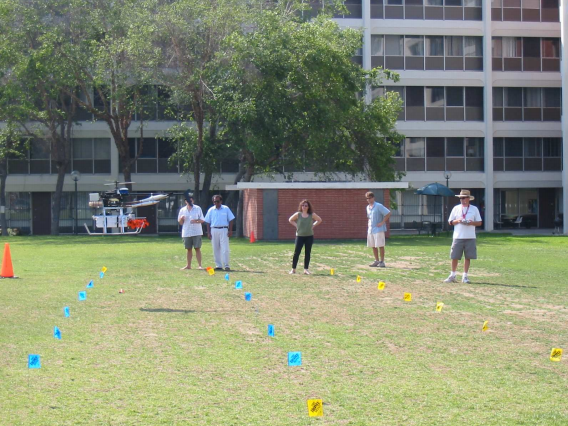
\includegraphics[width=0.3\textwidth]{figure1-1.1.png}}
%	\hspace{1cm}
%	\subfigure[]{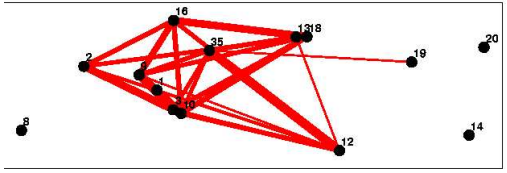
\includegraphics[width=0.3\textwidth]{figure1-1.2.png}}

%	\subfigure[]{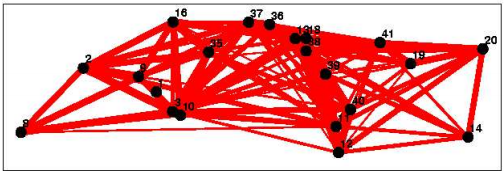
\includegraphics[width=0.3\textwidth]{figure1-1.3.png}}		
%	\bicaption[fig:SRR]{这里将出现在插图索引中}{中文题图}{Fig}{English caption}
%\end{figure*}
\begin{figure*}[!htbp]
	\begin{multicols}{2}
		
		\begin{center}
			\subfigure[直升机集中式控制拓扑网络]{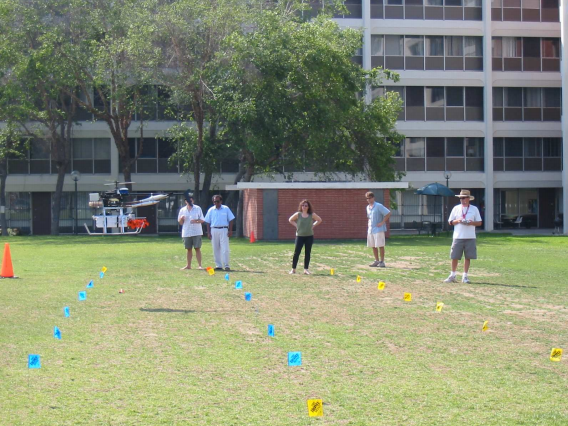
\includegraphics[width=6cm,height=4.8cm]{figure1-1.1.png}}
		\end{center}
		\begin{center}
			\subfigure[修复前的拓扑网络]{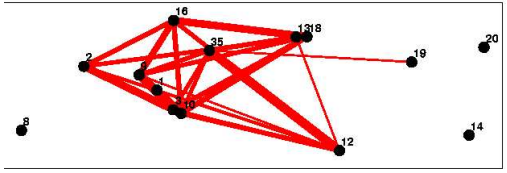
\includegraphics[width=5cm,height=1.7cm]{figure1-1.2.png}}
		\end{center}
		\begin{center}
			\subfigure[修复后的拓扑网络]{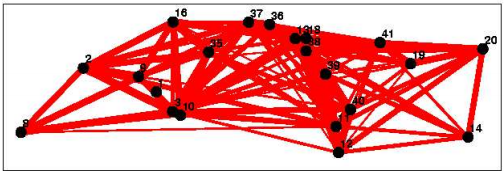
\includegraphics[width=5cm,height=1.7cm]{figure1-1.3.png}}
		\end{center}
	\end{multicols}
	\bicaption[fig:SRR]{利用无人机机进行集中式控制拓扑网络的直接自修复算法}{利用无人机机进行集中式控制拓扑网络的直接自修复算法}{Fig}{Autonomous deployment and repair of a sendor network using an unmanned aerial vehicle}
\end{figure*}

文献\parencite{Auto-holeDetection}中针对传感器网络覆盖问题进行了自修复的研究。文中主要针对网络覆盖中可能出现的空洞进行探测并修复。在算法执行过程中每个传感器节点与其他节点交换信息,多次交换信息后每个节点可以获得一个以它自身为中心的x-hop的邻居列表。即每一个节点能够获得拓扑网络中所有其他节点的信息,并计算出每个节点距离自己的跳数。如果出现空洞,则节点会根据自己的邻居列表选出一条修复路径,然后从所有的路径中选择一条效率最高的路径执行自修复。该算法需要每个节点都能够获得其他节点的信息,通信量比较大,且对每个节点的存储空间有所要求。若实现大规模节点的自修复则算法的时间和空间复杂度比较大,算法实现效率较低。

文献\parencite{Zhang2006Motion}针对多机器人编队网络的运动同步性进行自修复。当多机器人编队网络中出现机器人故障或者通信失效时,可能会影响整个网络的运动同步性。此时文中算法采用临时扩大机器人通信范围的方式,使得编队中所有机器人能够共享信息,从而直接选出合适的修复机器人进行自修复。修复过程如图1-2所示。
\begin{figure*}[!htbp]
	\begin{multicols}{2}
		\begin{center}
			\subfigure[]{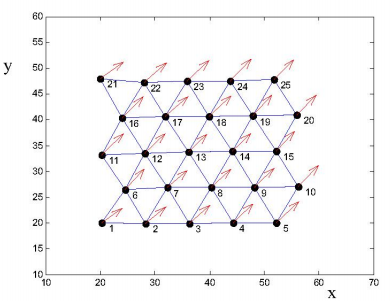
\includegraphics[width=6cm, height=4cm]{figure1-2.a.png}}
		\end{center}
		\begin{center}
			\subfigure[]{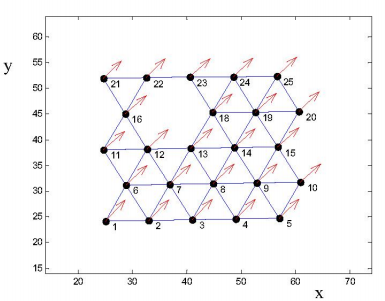
\includegraphics[width=6cm,height=4cm]{figure1-2.b.png}}
		\end{center}
		\begin{center}
			\subfigure[]{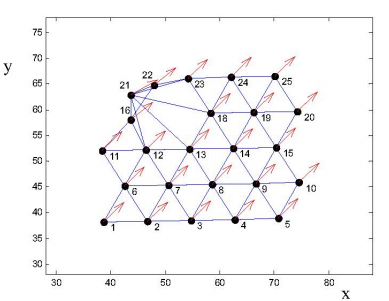
\includegraphics[width=6cm,height=4cm]{figure1-2.c.png}}
		\end{center}
		\begin{center}
			\subfigure[]{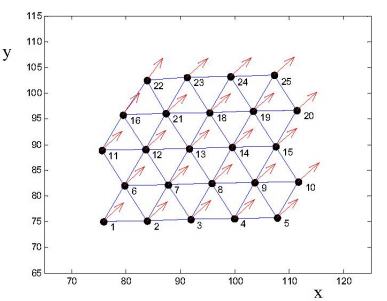
\includegraphics[width=6cm,height=4cm]{figure1-2.d.png}}
		\end{center}
	\end{multicols}
	\bicaption[fig:SRR]{多机器人编队网络运动同步性直接自修复}{多机器人编队网络运动同步性直接自修复}{Fig}{Directly self-healing for multi-robot formation motion synchronization.}	
\end{figure*}
由于出现机器人缺失后需要临时扩大机器人的通信范围,因此,算法不能算是完全分布式。并且多机器人的编队规模要收到传感器的最大通信距离的限制,不可能实现大规模机器人的编队控制,并且同样通信时间以及复杂度要随着编队规模的扩大呈指数型增长。

\subsection{密度自修复算法}
密度自修复算法主要应用在大量机器人进行自组装,形态生成或者区域覆盖等任务中。系统中的节点能够感知自身所处位置的密度,以此作为依据执行自修复算法,最终能够能够根据系统要求取得合理分布。文献\parencite{arbuckle2010self}中,作者仿照生物学纳米分子间信息交流的方式,研究了多智能体自主形态生成问题。在系统中已知一个几何形状,然后解析出几何形状的边集合,节点的有序集合。通过大量统一结构、统一编程的微小机器人执行分布式的形态生成算法可以构建出任意指定的形状。并且算法具有一定的容错机制,能够针对机器人失效,进行自修复。如图1-3所示。
\begin{figure}[!htbp]
	\centering
	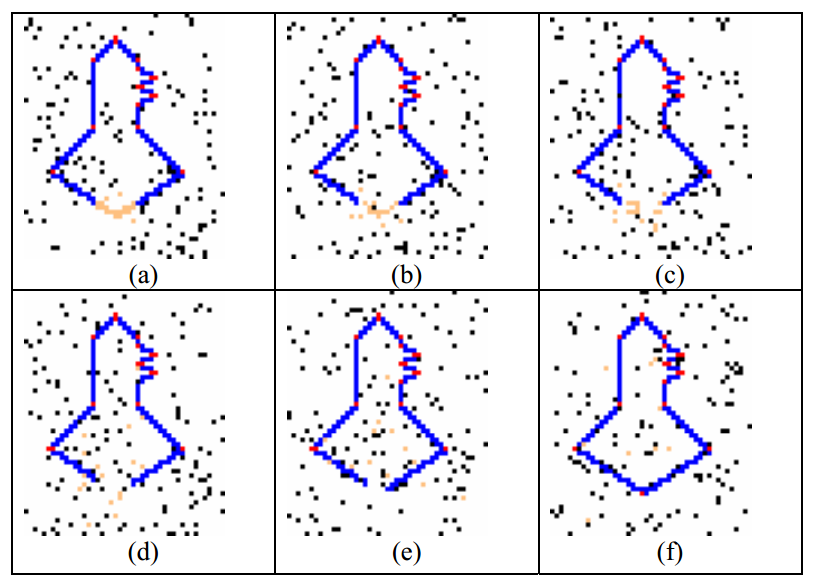
\includegraphics[width=10cm,height=6cm]{figure1-3.png}
	\bicaption[fig:SRR]{形态生成过程中机器人失效后的自修复}{形态生成过程中机器人失效后的自修复$^{[ ]}$}{Fig}{The structure recovers from the damage and self-repairs$^{[ ]}$}
\end{figure}
然而此算法的自修复过程具有一定的负面效应。即当机器人数量比较多,信息共享不完全时可能在系统中复制出两个完全一样的形状。

在文献\parencite{derbakova2011decentralized}中,作者研究了群机器人有效覆盖特定区域的算法。该算法能够实现群机器人针对某一区域的覆盖,并能对覆盖失效的情况进行自修复。系统中存在一个网关,负责所有机器人之间通信的中转。每个机器人通过与邻居通信间接与网关链接。在已知感兴趣区域的形状之后,机器人根据自身位置,结合密度信息执行分散算法,最终能够均匀覆盖该区域。并且在区域内某些机器人被移除后,系统能够自动感知缺失,并通过网关进行路径规划,调度其他机器人重新均匀覆盖此区域。如图1-4所示。
\begin{figure*}[!htbp]
	\begin{tabular}{cccc}
			\subfigure[]{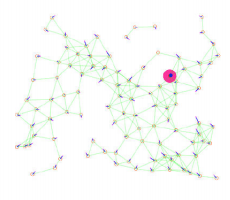
\includegraphics[width=4cm,height=5cm]{figure1-4.a.png}} &
			\subfigure[]{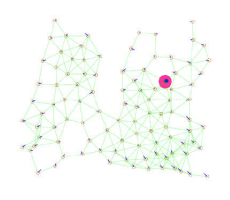
\includegraphics[width=4cm,height=5cm]{figure1-4.b.png}} &
			\subfigure[]{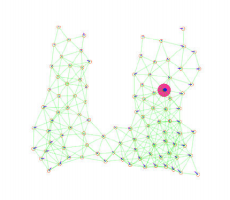
\includegraphics[width=4cm,height=5cm]{figure1-4.c.png}} &
			\subfigure[]{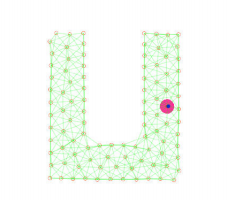
\includegraphics[width=4cm,height=5cm]{figure1-4.d.png}} \\
			\subfigure[]{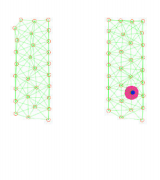
\includegraphics[width=4cm,height=5cm]{figure1-4.e.png}} &
			\subfigure[]{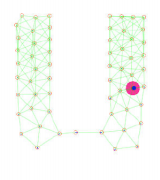
\includegraphics[width=4cm,height=5cm]{figure1-4.f.png}} & 
			\subfigure[]{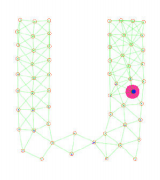
\includegraphics[width=4cm,height=5cm]{figure1-4.g.png}} &
			\subfigure[]{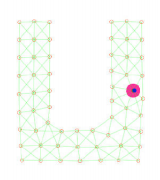
\includegraphics[width=4cm,height=5cm]{figure1-4.h.png}} \\
	\end{tabular}
	\bicaption[fig:SRR]{多移动机器人区域覆盖网络连接自修复算法}{多移动机器人区域覆盖网络连接自修复算法}{Fig}{Coverage and repair algorithm for multi-robot systems}
\end{figure*}
\subsection{递归自修复算法}
递归自修复算法利用节点或机器人之间局部交互和网络拓扑切换实现自修复。在文献\parencite{abbasi2009movement}中Abbassi等人针对无线传感器执行器网络(Wireless Sensor and Actor Networks, WSANs)中节点失效影响网络连通性的问题,提出了DARA(Distributed Actor Recovery Algorithm)算法。DARA算法针对不同的网络拓扑分为DARA-1C和DARA-2C两个版本。DARA-1C算法用于维持和修复网络的一阶连通性。算法通过心跳机制检测网络中的节点丢失。当节点出现丢失时从丢失节点的邻居中根据节点的度、离缺失节点的距离大小、自身ID号等条件选取最佳候选修复节点。网络中每个节点维持二跳邻居信息,主要针对网络中割点(cut-vertex)丢失导致网络分裂成两个或多个部分的问题进行修复。如图1-5所示。
\begin{figure*}[!htbp]
	\centering
	\begin{tabular}{ccc}
		\subfigure[]{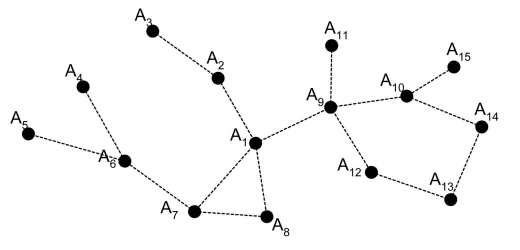
\includegraphics[width=5cm,height=3cm]{figure1-5.a.png}}
		\subfigure[]{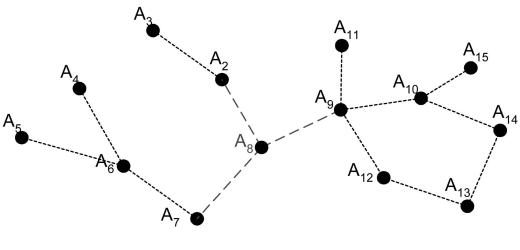
\includegraphics[width=5cm,height=3cm]{figure1-5.b.png}}
		\subfigure[]{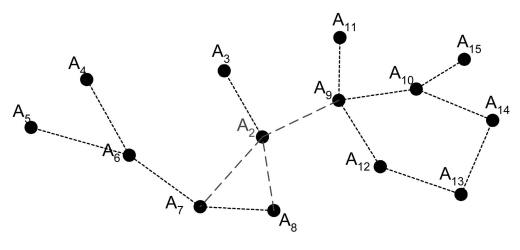
\includegraphics[width=5cm,height=3cm]{figure1-5.c.png}}
	\end{tabular}
	\bicaption[fig:SRR]{使用DARA-1C算法实现传感器网络连接自修复}{使用DARA-1C算法实现传感器网络连接自修复}{Fig}{Using DARA-1C to repair the connectivity of WSANs}
\end{figure*}

DARA-2C算法目的是维持网络的2阶连通性。可以实现网络外围节点丢失的自修复。算法的实现方式与DARA-1C类似,但主要是针对网络边缘节点进行自修复,目的是防止出现割点(cut-vertex)。修复算法只考虑是否维持2阶连通性。修复过程如图1-6所示。
\begin{figure}[!htbp]
	\centering
	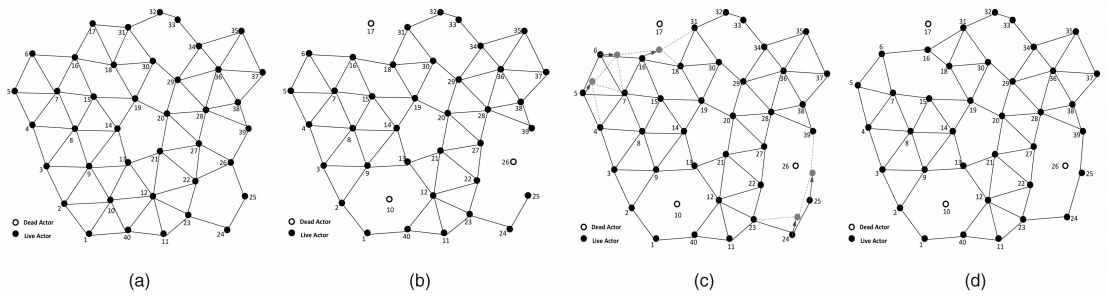
\includegraphics[width=15cm,height=4cm]{figure1-6.png}
	\bicaption[fig:SRR]{使用DARA-2C算法实现传感器网络2阶连通性自修复}{使用DARA-2C算法实现传感器网络2阶连通性自修复}{Fig}{Using DARA-2C to repair 2-connectivity of WSANs}
\end{figure}

在文献\parencite{younis2010localized}中,同样针对传感器网络连通性问题,Younis等人提出了RIM(Recovery through Inward Motion)自修复算法。该算法主要是在节点出现缺失之后,缺失节点的所有邻居节点全部向缺失节点的位置移动,直至重新建立连接。缺失节点的邻居节点移动后若如出现新的空缺则由其邻居继续执行RIM算法进行自修复,直至整个网络保持连通。如图1-7所示。该算法只考虑网络的连通性,不考虑拓扑结构的变化。
\begin{figure}
	\centering
	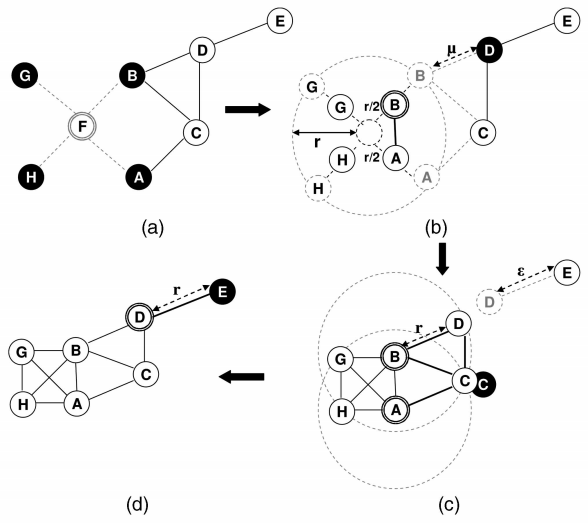
\includegraphics[width=9cm,height=8cm]{figure1-7.png}
	\bicaption[fig:SRR]{RIM算法自修复过程}{RIM算法自修复过程}{Fig}{The self-healing process of RIM algorithm}
\end{figure}

综上所述,前人关于自修复的算法几乎都是针对网络的联通性。然而类似于多机器人协同搬运这样的任务,需要多机器人能够保持特定的队形并且对编队的运动同步性要求较高。显然上述算法都无法适用于针对多机器人编队运动同步性的自修复。因此如何设计一种性能良好的针对多机器人编队网络运动同步性的自修复算法是值得思考和亟需解决的问题。

\section{本文研究内容及组织框架}
本文针对多机器人编队网络中存在机器人缺失,从而导致整个编队运动同步性下降的问题,提出了一种分布式的递归自修复算法。该算法能够实现同步性改善全局最优,通过在编队网络中构建稳定的梯度分布可以找到一条实现同步性改善全局最优的修复路径,并且该修复路径包含修复机器人个数最少,机器人运动的总距离最短。针对本文算法,不仅利用仿真验证了算法的理论可行性和有效性,而且还设计了包括多机器人空间定位系统,通信系统,运动控制系统在内的自修复实验平台。在此平台下开展了实验,验证了算法的现实可行性和可操作性。

本文主要贡献如下:\\
\indent 1) 提出了一种分布式的多机器人编队自修复算法。该算法在编队中出现机器人缺失后不仅修复了编队队形还能够实现同步性改善全局最优。\\
\indent 2) 在本文算法中引入梯度,并设计了一中新的梯度扩散与更新机制,从而实现同步性改善全局最优的同时保证修复路径最短,修复机器人个数最少。\\
\indent 3) 设计了仿真验证算法在同步性改善、修复机器人个数、修复机器人运动距离等指标的考量。\\
\indent 4) 设计了多机器人编队自修复实验平台。平台包括基于Vicon的多功能可扩展的空间定位系统、多机器人的通信系统以及机器人底层运动控制系统。

本文各章节简介如下:\\
\indent 第一章,\\
\indent 第二章,\\
\indent 第三章,\\
\indent 第四章,\\
\indent 第五章,\\




\chapter{编队网络模型和拓扑分析}
\label{chap:2}

\section{机器人编队网络模型}
在多机器人编队控制过程中,每个机器人个体都具有自主行动能力。尤其在实现分布式控制算法时,每个个体机器人需要具有独立的决策与执行能力。因此,机器人个体运动模型对编队的控制至关重要。另外在应用编队控制算法对整个编队系统进行控制从而实现特定任务时,对整体编队网络拓扑模型的掌握也是必不可少。编队网络拓扑模型是对整体编队网络拓扑分析与拓扑控制的基础\supercite{张飞2010}。

\subsection{机器人个体运动模型}
假设在$N$维空间内,机器人$i$的位置和速度分别表示为$p_i \in R^N$和$v_i \in R^N$。则机器人个体运动模型可以表示如下:\\
\begin{equation}
	\left\{
	\begin{aligned}
		\dot{p_i} & = v_i \\
		\dot{v_i} & = u_i^e + u_i^o
	\end{aligned}
	, i=1,2,\dots,n,
	\right.
\end{equation}
其中$u_i^e$表示外部对机器人的控制输入,$u_i^o$表示其他机器人对机器人$i$的影响。$u_i^e$可简单表示为:\\
\begin{equation}
	u_i^e = f(p_i,v_i), i=1,2,\dots,n
\end{equation}
若考虑障碍环境中,则$u_i^e$可表示为:\\
\begin{equation}
	u_i^e = f_a(p_i,v_i) + f_r(p_i,v_i), i=1,2,\dots,n
\end{equation}
其中,$f_a(p_i,v_i)$为目标对机器人的吸引力,$f_r(p_i,v_i)$为障碍物对机器人的排斥力。如果已知目标点的位置$T$和机器人当前位置的期望速度$v(t)$,则$f_a(p_i,v_i)$可以表示为:\\
\begin{equation}
	f_a(p_i,v_i) = a_a(T-p_i) + a_m(v(t)-v_i), i=1,2,\dots,n
\end{equation}
$a_a,a_m$分别为位置和速度的增益系数,且满足$a_a,a_m > 0$。

假设环境中存在一球形障碍物,其中心点位于$O$,半径为$r_0$,则排斥力$f_r(p_i,v_i)$可表示为:\\
\begin{equation}
	f_r(p_i,v_i) = \begin{cases}
		\frac{a_0}{{(\lvert\lvert p_i-O \rvert\rvert -r_0)}^2} \cdot \vec{r}_t, & \lvert\lvert O-p_i \rvert\rvert \leq r_0 + R_s \\
		0, &  \lvert\lvert O-p_i \rvert\rvert > r_0 + R_s
	\end{cases}
\end{equation}
其中$a_0$为排斥系数,$R_s$为人为设置的障碍物有效作用半径。$\vec{r}_t$为排斥力的方向,即$\vec{r}_t = \vec{Op_i}/\lvert\lvert\vec{Op_i}\rvert\rvert$。

\subsection{多机器人编队网络拓扑模型}
本文的拓扑结构采用基于图论的网络拓扑。假设机器人编队中有$n$个机器人,$n$个机器人组成的编队网络用$G=(V,E)$表示,其中$V$表示图中节点的集合,$E$表示节点间边的集合。每个节点$v_i\in V, i=1,2,\dots,n$表示机器人$i$, $(v_i,v_j)\in E, i,j=1,2,\dots,n$表示机器人$i,j$之间的链接。利用矩阵$A=(a_{ij}),a_{ij} \in R^{n \times n}$表示网络拓扑的耦合关系,其中\\
\begin{equation}
	a_{ij}=a_{ji} =
	\begin{cases}
		1, & (v_i,v_j) \in E \\
		0, & (v_i,v_j) \notin E
	\end{cases}
	, i,j = 1,2,\dots\dots,n, i \neq j
\end{equation}
$a_{ij} = a){ji} = 1$ 表示机器人$i,j$之间存在有效链接,否则不存在链接。耦合矩阵对角线上的元素$a_{ij} = -\sum_{i=1,i \neq j}^n a_{ij}$。规定与机器人$i$存在有效连接的机器人属于机器人$i$的邻居。则定义机器人$i$的邻居集合$N_e(i)$为:\\
\begin{equation}
	N_e(i) = \left\{ \forall j, j \neq i \wedge a_{ij}=1 \right\}
\end{equation}
机器人$i$的度为:\\
\begin{equation}
	d_i = \sum_{j \in N_e(i)} a_{ij}
\end{equation}
由此可知,耦合矩阵对角线上的元素$a_{ii} = -d_i$。

多机器人编队网络拓扑多采用$K$邻居模型\supercite{xue2004number}描述。在K邻居模型中,每个机器人的度$d_i \leq K, i=1,2, \dots ,n$。图2-1展示了几种常见的$K$邻居网络拓扑模型。

\begin{figure*}[!htbp]
	\centering
	\begin{tabular}{lr}
		\subfigure[K=3]{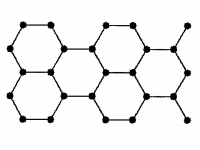
\includegraphics[width=5cm,height=4cm]{chapter2/figure2-1a.png}} &
		\subfigure[K=4]{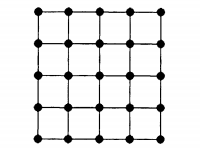
\includegraphics[width=5cm,height=4cm]{chapter2/figure2-1b.png}} \\
		\subfigure[K=6]{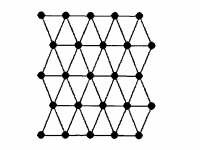
\includegraphics[width=5cm,height=4cm]{chapter2/figure2-1c.png}} &
		\subfigure[K=8]{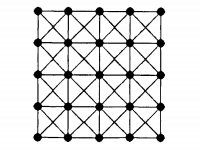
\includegraphics[width=5cm,height=4cm]{chapter2/figure2-1d.png}} \\
	\end{tabular}
\end{figure*}


\chapter{同步性改善全局最优的递归自修复算法}

\section{自修复算法目标}
根据上文所述,当多机器人编队中度较高的机器人出现缺失时,会导致编队同步性下降。假设在图\ref{fig:修复路径对比}中,空缺位置表示出现机器人缺失,记缺失机器人为$R_f$,则缺失机器人的度${R_f}.Deg = 6$。由引理\ref{lem:degree_syn}可知。若用度小于$R_f.Deg$的机器人修复此缺失机器人,则会提高编队的同步性。若最终修复机器人为$R_r$,度为$R_r.Deg$。则$R_f.Deg-R_r.Deg$的值越大,同步性改善效果越好。
%因此,本文目标之一是用编队中度最小的机器人去修复缺失机器人,使得同步性改善效果最优。
\begin{figure}[!htbp]
	\centering
	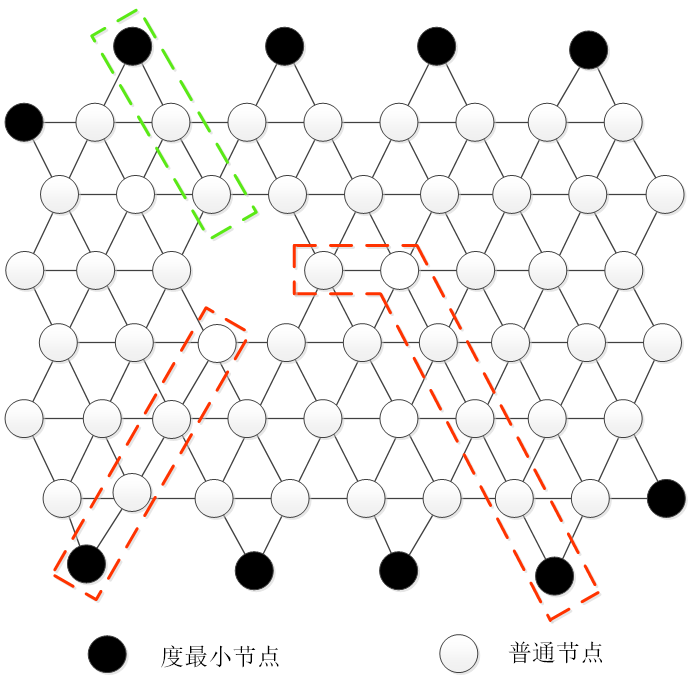
\includegraphics[width=8cm,height=8cm]{chapter3/figure3-1.png}
	\bicaption[fig:修复路径对比]{不同修复路径对比}{不同修复路径对比}{Fig}{The comparation of different repairing paths.}
\end{figure}

如何找到一条从缺失机器人到度最小机器人的修复路径是本文算法中主要解决的问题。在这里\textbf{修复路径}定义为从缺失机器人邻居中的某个机器人到编队中度最小机器人所经过的机器人序列$\{R_1,R_2,\dots,R_{k-1},R_k\}$。修复路径上的机器人成为修复机器人,其中$R_1$为缺失机器人邻居中的某个机器人,$R_k$为编队中某个度最小的机器人。\textbf{修复路径的长度}定义为修复路径中包含的修复机器人的个数。在图\ref{fig:修复路径对比}中,每一个虚线框中的机器人序列都属于一条修复路径。从图中可以看到不同的修复路径包含的修复机器人个数不同。定义包含修复机器人个数最少的修复路径为\textbf{最优修复路径},图中绿色虚线框内的修复路径即为一条最优修复路径。如果一条修复路径中的修复机器人序列为$\{R_1,R_2,\dots,R_{k-1},R_k\}$,则本文采用的递归自修复过程如下:\\
\indent (1)从缺失机器人的邻居中选择一个修复机器人$R_1$,$R_1$去填补缺失机器人留下的空缺位置,并与缺失机器人邻居重新建立。\\
\indent (2)$R_1$从其邻居中选择一个修复机器人$R_2$用来填补$R_1$移动后留下的空缺位置,并与$R_1$的邻居重新建立连接。\\
\indent (3)重复上述过程,直到编队中的度最小机器人$R_k$填补了$R_{k-1}$留下的空缺位置。\\
第(3)步结束后,整个修复机器人序列的递归自修复过程结束。在这一过程中,修复机器人的空间位置和网络邻居变化如下:\\
空间位置变化:
\begin{equation}
	P_{R_i} = 
	\begin{cases}
		P_{R_f}, & i=1 \\
		P_{R_{i-1}}, & 1 < i \leq k
	\end{cases}
\end{equation}
网络邻居变化:\\
\begin{equation}
	N_e(R_i) = 
	\begin{cases}
		N_e(R_f) - R_i + R_{i+1}, & i = 1 \\
		N_e(R_{i-1}) - R-i + R_{i+1}, & 1<k \leq k
	\end{cases}
\end{equation}

%本文采用上述递归自修复方式实现自修复过程,编队中机器人无法直接确定距离缺失机器人最近的度最小机器人在哪里。所以本文算法另一目标是找到一条最优的修复路径。
综上所述,当多机器人编队中机器人缺失时,本文自修复算法实现目标如下:\\
\indent\indent 1) 修复编队网络拓扑结构。\\
\indent\indent 2) 实现同步性改善全局最优。\\
\indent\indent 3) 自修复过程实现完全分布式,且修复路径最优。\\

本文算法的实现主要基于以下假设:\\
\indent\indent 1) 机器人缺失后,整个编队网络仍然保持连通。\\
\indent\indent 2) 机器人之间的通信速率足够快,从而忽略通信时间消耗。\\
\indent\indent 3) 缺失机器人不影响其他机器人的运动。

\section{梯度的引入与分析}
根据前人的研究,梯度常被用于通过邻居之间的交互估计分布式距离的一种手段\supercite{SciencePaper,nagpal2003organizing,stoy2006using,rubenstein2012kilobot,meng2011autonomous,terada2008automatic},多应用于有限通信范围下的多传感器网络\supercite{nagpal2003organizing}以及多机器人自组织行为\supercite{SciencePaper,stoy2006using}等问题。主要是通过个体间的局部交互来控制整体。文献\parencite{SciencePaper,stoy2006using,rubenstein2012kilobot,terada2008automatic}中,首先定义一个梯度种子节点,由种子节点产生一个初始梯度值,接下来梯度值从种子节点开始扩散,邻居节点接收到扩散的梯度信息后更新自己的梯度信息,一般情况是如果接受到的梯度小于自身已有的梯度值(自身梯度值初始化为一个很大的数),则更新自身梯度值,否则维持自身梯度值不变。接下来再将自身保持的梯度值向邻居扩散,重复此过程,最终整个网络会形成稳定的梯度分布。每个机器人利用自身的梯度信息便可以知道自己与梯度种子节点的距离。图\ref{fig:Gradient_Sample}展示的是文献\parencite{SciencePaper}中的梯度应用示例。在多机器人自组织行为中,预先指定一个梯度种子节点的梯度值以及它的全局坐标,利用梯度扩散与更新过程在网络中形成稳定的梯度分布,在扩散与更新过程中,每个机器人只与它相邻的机器人通信。最终每个机器人根据自身的梯度值以及梯度种子节点的全局坐标估计出自己的全局坐标,从而完成自组织任务。
\begin{figure}[!htbp]
	\centering
	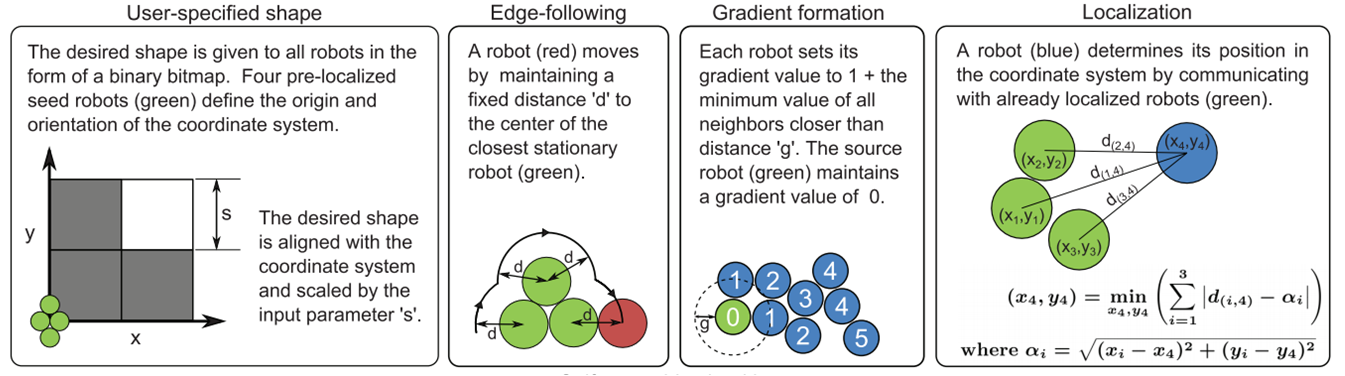
\includegraphics[width=12cm,height=3cm]{chapter3/figure3-2.png}
	\bicaption[fig:Gradient_Sample]{应用梯度实现多机器人自组织行为}{应用梯度实现多机器人自组织行为}{Fig}{Using Gradient to implement multi-robot self-assembly behaviors.}
\end{figure}

为对比有无梯度信息在多机器人编队自修复中的差别,在本团队前期工作中\supercite{张飞2008移动机器人覆盖问题的研究,liu2015gradient,居建军2015多机器人编队自修复算法设计与实现}分别实现了无梯度和有梯度的多机器人编队自修复算法。在文献\parencite{张飞2008移动机器人覆盖问题的研究}中,编队中机器人缺失后仅根据邻居机器人的度的信息选择修复机器人,选取规则为:\\
\indent 1) 如果缺失机器人$R_f$的邻居$R_j \in N_e(R_f)$的度小于$R_f$的度,即$R_j.Deg \leq R_f.Deg$,则机器人$R_j$成为缺失机器人$R_f$的候选修复机器人。所有满足条件的候选修复机器人组成集合:
\begin{equation}
	C(R_f) = \{ R_j | R_j.Deg \leq R_f.Deg, R_j \in N_e{R_f} \} 
\end{equation} 
\indent 2) 在集合$C(R_f)$中选择度最小的机器人作为缺失机器人$R_f$的修复机器人,如果存在多个度最小机器人,则随机选择一个作为修复机器人。

本文中称此算法为随机递归自修复算法。图\ref{fig:Random_self-healing}中展示了在多机器人编队拓扑中出现一个机器人丢失,应用随机自修复算法进行修复的几种情况。
\begin{figure*}[!htbp]
	\centering
	\begin{tabular}{cc}
		\subfigure[]{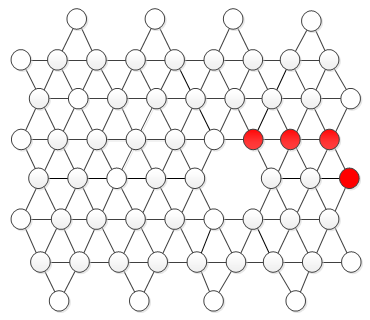
\includegraphics[width=4cm,height=3.5cm]{chapter3/figure3-3a.png}} & 
		\hspace{2cm}
		\subfigure[]{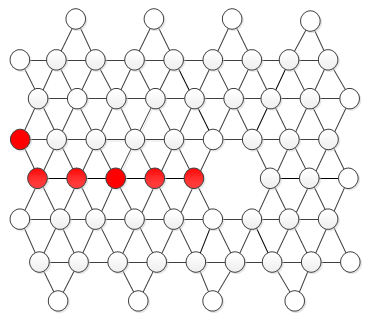
\includegraphics[width=4cm,height=3.5cm]{chapter3/figure3-3b.png}} \\

		\subfigure[]{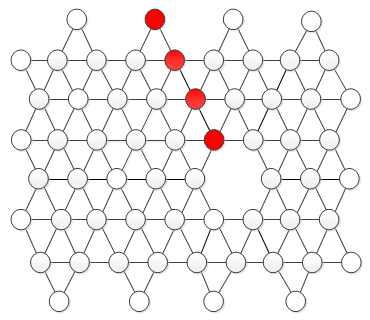
\includegraphics[width=4cm,height=3.5cm]{chapter3/figure3-3c.png}} & 
		\hspace{2cm}
		\subfigure[]{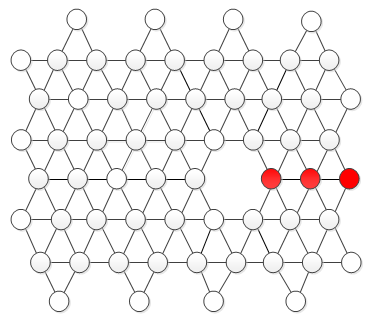
\includegraphics[width=4cm,height=3.5cm]{chapter3/figure3-3d.png}} 
	\end{tabular}
	\bicaption[fig:Random_self-healing]{随机递归自修复算法}{随机递归自修复算法,空缺位置表示此处机器人丢失,红色节点表示修复机器人}{Fig}{Random-based recursive self-healing algorithm.}
\end{figure*}

从图中可以看出随机递归自修复算法在实现自修复时选出的修复路径有很大的随机性,且不同的修复路径性能差异较大。造成这种现象的原因主要是在修复机器人选取规则2中,当存在多个满足条件的候选修复机器人时随机选择其中一个,由此对修复路径造成很大的随机性。

为避免在自修复中引入过大的随机性,本研究团队在之前工作中引入梯度,大大降低了随机性,提高了自修复算法的性能。如图\ref{fig:Gradient_self-healing}所示,是在编队网络中引入梯度,形成稳定的梯度分布,算法中与前人不同的是并不事先指定一个梯度种子节点,而是节点根据自己在拓扑网络中邻居数量判断自己是否为梯度种子节点(又称为梯度源节点)。即梯度源节点的定义如下:
\begin{defn}
	\label{defn:gradient_source}
	若编队中机器人$R_i$的度满足:\\
	\begin{equation}
		\forall R_j \in N_e(R_i), R_j.Deg > R_i.Deg
	\end{equation}
	则称机器人$R_i$为梯度源节点。
\end{defn}
修复机器人选取规则为:\\
\indent 1)在缺失机器人$R_f$的邻居中选择度不大于缺失机器人度的机器人作为候选修复机器人。\\
\indent 2)选择候选修复机器人集合中度最小的机器人作为修复机器人。\\
\indent 3)如果存在多个度最小的候选修复机器人,则选择其中梯度值最小的机器人作为修复机器人。\\
\indent 4)如果存在多个度最小且梯度值最小的候选修复机器人,则从中随机选择一个机器人作为修复机器人。\\
图\ref{fig:Gradient_self-healing}是引入梯度后的自修复情况,本文称此算法为基于梯度的递归自修复算法。
\begin{figure*}[!htbp]
	\centering
	\begin{tabular}{cc}
		\subfigure[]{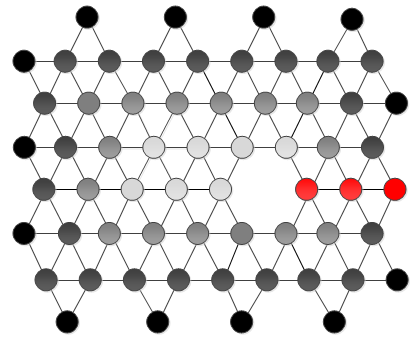
\includegraphics[width=4cm,height=3.5cm]{chapter3/figure3-4a.png}} & 
		\hspace{2cm}
		\subfigure[]{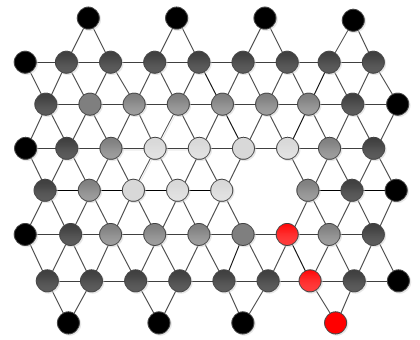
\includegraphics[width=4cm,height=3.5cm]{chapter3/figure3-4b.png}} \\
		
		\subfigure[]{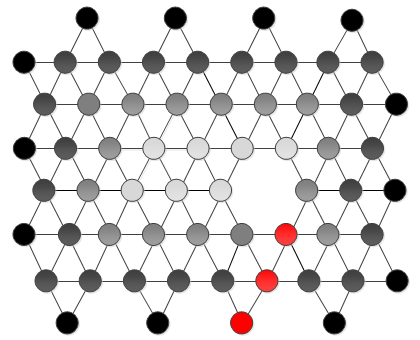
\includegraphics[width=4cm,height=3.5cm]{chapter3/figure3-4c.png}} & 
		\hspace{2cm}
		\subfigure[]{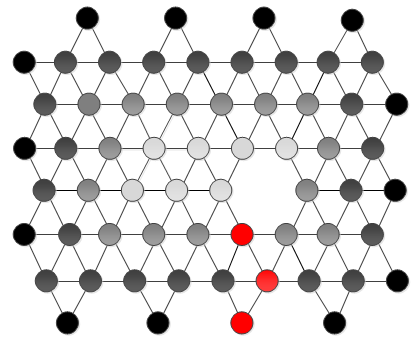
\includegraphics[width=4cm,height=3.5cm]{chapter3/figure3-4d.png}} 
	\end{tabular}
	\bicaption[fig:Gradient_self-healing]{基于梯度的递归自修复算法}{基于梯度的递归自修复算法,颜色的深浅表示梯度值的大小,颜色越深梯度值越小。黑色节点为梯度源节点。空缺位置表示此处机器人丢失,红色节点表示修复机器人}{Fig}{Gradient-based recursive self-healing algorithm, the shade means different gradient value, the deeper the color, the bigger the gradient value, the vacancy means failure robot and red nodes means repairing robots.}
\end{figure*}
从图中可以看到,引入梯度后修复路径的随机性降低很多,且修复路径是一条最短的修复路径。但是这里存在局部极小问题,在图\ref{fig:Gradient_self-healing}(a)中修复机器人序列中最后的梯度源节点机器人的度并不是全局最小。因此根据引理\ref{lem:degree_syn},同步性改善并不是全局最优。

本文借鉴前人的做法,在多机器人编队自修复算法中利用梯度分布式估计机器人与度最小机器人的距离,从而找到最优的修复路径。但为避免局部极小的问题,编队在梯度扩散与更新过程中所传播的信息不只是梯度信息还包括梯度源节点的度的信息,从而将局部度极小节点而非全局度最小节点更新,下文会具体分析这一过程。定义\textbf{梯度源节点的度}为机器人梯度值的扩散起点的梯度源节点的度的值。

\section{同步性改善全局最优自修复算法}

\subsection{算法框架}
总结前人研究的经验,本文设计了一种能够实现同步性改善全局最优的递归自修复算法。本文算法可以在编队中每个机器人个体上独立运行,从而实现完全分布式控制。本文算法主要根据在自修复过程中个体机器人本身在不同情况下所执行的任务的不同分为5种状态,分别为初始状态、梯度源节点状态、非梯度源节点状态、候选修复状态以及修复状态。在多机器人编队开始运行之后,编队中的机器人首先处于初始状态,通过执行梯度源节点生成算法判断自身是否为梯度源节点,若满足满足梯度源节点条件,则状态转移到梯度源节点状态,否则,状态转移到非梯度源节点状态。处于梯度源节点状态和非梯度源节点状态的机器人进行梯度的更新与扩散,最终在编队网络中形成稳定的梯度分布。编队在出现机器人缺失后执行修复的过程是建立在稳定的梯度分布基础之上的。形成稳定的梯度分布之后,当编队中出现机器人缺失时,缺失机器人的邻居检测到邻居中出现机器人缺失,则由当前状态转移到候选修复状态,所有处于候选修复状态下的机器人采用本文提出的竞选机制进行竞选以决出最终的修复机器人。竞选胜出的机器人状态转移到修复状态,处于修复状态的机器人将修复状态进行传递,知道度最小机器人状态转移到修复状态。图\ref{fig:FSM}的FSM图描述了机器人各个状态之间的转换关系。下文会结合编队拓扑给出各个状态更详细的分析。
\begin{figure}[!htbp]
	\centering
	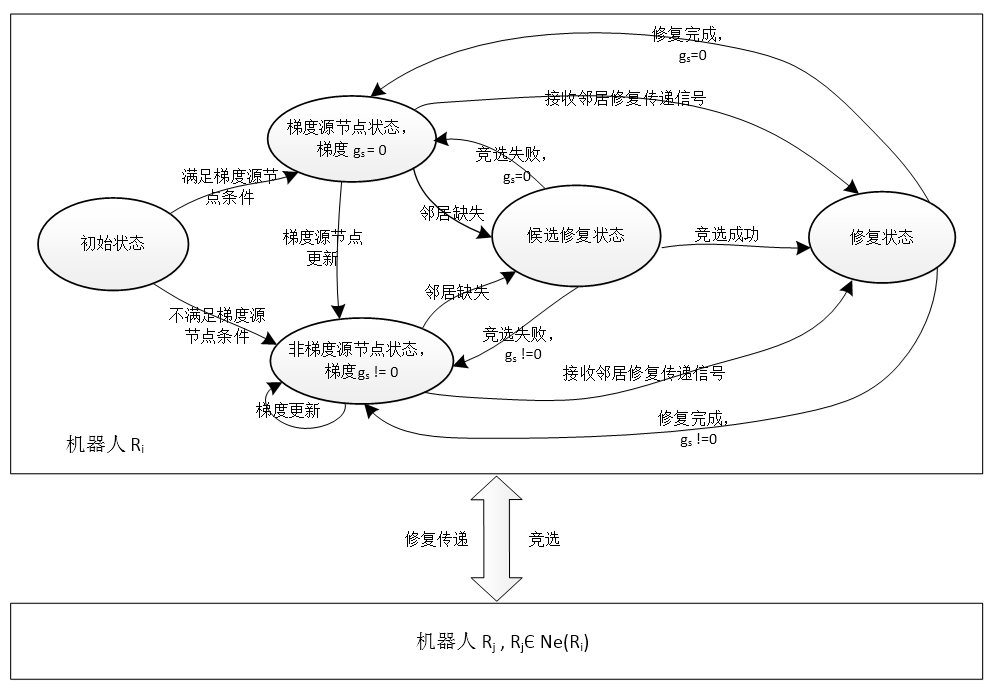
\includegraphics[width=14cm,height=10cm]{chapter3/figure3-5.png}
	\bicaption[fig:FSM]{同步性改善全局最优自修复算法状态转换图}{同步性改善全局最优自修复算法状态转换图}{Fig}{The FSM for the proposed algorithm.}
\end{figure}

\subsection{初始状态}
当编队刚开始运行时,所有机器人最开始都处于初始状态。在这一状态下机器人会执行相应的初始化工作,初始化的工作之一就是将自身的梯度值以及梯度源节点的度的值设置为一个很大的值$N_A$,用$Gra$表示机器人的梯度值,$DS$表示机器人的梯度源节点的度的值,则$Gra=N_A, DS=N_A$。接下来在这一状态下机器人的主要工作是判断自身是否为梯度源节点。根据梯度源节点的定义,判断自身是否为梯度源节点的伪代码如下:\\
\begin{algorithm}
	\caption{判断是否为梯度源节点}
	\label{IsSourceNode}
	\begin{algorithmic}[1]
		\Require 邻居集合$NeighborList[]$
		\Ensure $Ret$,是否为梯度源节点,$Ret \leftarrow true$是梯度源节点,$Ret \leftarrow false$不是梯度源节点
		\Function{IsSourceNode}{$NeighborList[]$}
			\State $Ret \gets false$
			\For {$d_i \ in \ NeighborList[]$}
				\If {$d_i.Deg \leq Deg$}
					\State $Ret \gets false$
				\EndIf
			\EndFor 
			\State \Return{$Ret$}
		\EndFunction
	\end{algorithmic}	
\end{algorithm}
执行上述程序之后,如果判断自身为梯度源节点则将状态转移到梯度源节点状态,如果判断不是梯度源节点,则将状态转移到非梯度源节点状态。图\ref{fig:initial_status}显示了编队拓扑网络中不同机器人节点执行判断是否为梯度源节点的程序后的判断结果。
\begin{figure}[!htbp]
	\centering
	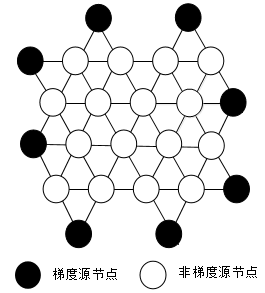
\includegraphics[width=6cm,height=6cm]{chapter3/figure3-6.png}
	\bicaption[fig:initial_status]{梯度源节点的分布}{梯度源节点的分布}{Fig}{The distribution of gradient source node.}
\end{figure}

\subsection{梯度源节点状态与非梯度源节点状态}
处于梯度源节点状态的机器人首先会将自身的梯度值置零,将梯度源节点的度设置成自身的度的大小,即$Gra=0; DS = Deg$。接下来处于梯度源节点状态的机器人会将自身梯度值$Gra$,梯度源节点的度值$DS$封装成一个数据对$P = [Gra,DS]$,然后将此数据对发送给自己的邻居机器人,由此触发整个编队的梯度扩散过程。根据图\ref{fig:initial_status}中的拓扑结构可知,梯度源节点的邻居包含非梯度源节点状态的机器人。又梯度扩散时整个编队拓扑层面的行为,因此梯度扩散过程是由编队中所有机器人参与完成的,梯度源节点触发梯度扩散过程,非梯度源节点传递梯度。因此下面描述的梯度扩散过程是属于梯度源节点状态和非梯度源节点状态下的机器人的共同行为。前文提到过,在梯度源节点生成时会产生局部极小的问题。如图\ref{fig:initial_status}所示,在初始状态下生成的梯度源节点部分度为2,部分度为3,并非全部拥有全局最小度。因此若在当前梯度源节点的分布下形成稳定的梯度分布,则无法保证最终的修复结果达到同步性改善全局最优。这也是文献\parencite{liu2015gradient}中取得效果。这也是本文算法引入梯度源节点的度的原因。本文算法会在梯度扩散过程中根据梯度源节点的度的信息判断当前梯度源节点是否为全局度最小节点,如果不是全局度最小节点,则将其更新为非梯度源节点,状态转移到非梯度源节点状态。经过这样的更新之后,编队中的梯度源节点全部拥有全局最小度,所有节点的梯度值也全部是由全局度最下节点扩散而来。由此可知,在梯度扩散过程中包含两个可能行为,即梯度的更新与梯度源节点的更新,而梯度源节点的更新只可能发生在梯度源节点状态下的机器人。由于这两个行为在梯度扩散过程中同时存在,因此以下梯度扩散公式包含上述两个行为。

梯度扩散公式如下:\\
${ \forall R_j \in N_e(R_i), \delta \geq 0, \Delta \geq 0, \Delta \gg \delta,}$ \\
\begin{equation}\scriptsize
	P_i(t) = 
	\begin{cases}
		\vspace{0.5cm}
		\left[
		\begin{array}{c}
			R_j.Gra(t-1) + \Delta \\
			R_j.DS(t-1)
		\end{array}
		\right], & 
		\begin{array}{l}
			R_i.DS(t-1) > R_j.DS(t-1) \vee \\
			(R_i.DS(t-1) = R_j.DS(t-1) \wedge R_i.Gra(t-1) +\delta > R_j.Gra(t-1) + \Delta)
		\end{array} \\
		
		\left[
		\begin{array}{c}
		R_i.Gra(t-1) + \delta \\
		R_i.DS(t-1)
		\end{array}
		\right], & 
		\begin{array}{l}
			R_i.DS(t-1) < R_j.DS(t-1) \vee \\
			(R_i.DS(t-1) = R_j.DS(t-1) \wedge R_i.Gra(t-1) +\delta \leq R_j.Gra(t-1) + \Delta)
		\end{array}		
	\end{cases} 
\end{equation}
式中:\\
\indent $t$ —— 梯度传播的次数,一个单位代表邻居间传递一次消息。\\
\indent $P_i(t)$ —— $t$次梯度传播后,机器人$R_i$的信息对。\\
\indent $R_j.Gra(t-1)$ —— $t-1$次梯度传播后机器人$R_j$的梯度值。\\
\indent $R_j.DS(t-1)$ —— $t-1$次梯度传播后机器人$R_j$的梯度源节点的度。\\
\indent $R_i.Gra(t-1)$ —— $t-1$次梯度传播后机器人$R_i$的梯度值。\\
\indent $R_i.DS(t-1)$ —— $t-1$次梯度传播后机器人$R_i$的梯度源节点的度。\\
\indent $\delta$ —— 机器人一次梯度传播后梯度增量。\\
\indent $\Delta$ —— 邻居间扩散的梯度增量。

1.梯度更新:\\
\indent 若机器人接收到的信息对中梯度源节点的度值小于自身梯度源节点的度值,则将自身的梯度源节点的度值更新为接收到的梯度源节点的度值,自身梯度值更新为接收到的梯度值加上邻居间的梯度增量。如果接收到的信息对中梯度源节点的度值等于自身梯度源节点的度值,则比较梯度值,若自身梯度值大于信息对中的梯度值加上邻居间扩散的梯度增量,则将自身梯度值更新为信息对中的梯度值与梯度增量的和。

2.梯度源节点更新:\\
\indent 若自身为梯度源节点,且接收到的信息对中梯度源节点的度值小于自身的度值,则将自身状态转移到非梯度源节点状态,并更新相应的梯度源节点的度和梯度值。

梯度扩散算法的伪代码如下:\\
\begin{algorithm}
	\caption{梯度扩散算法}
	\label{algorithm:gradient_diffusion}
	\begin{algorithmic}[1]
		\Require $R_j.Gra \leftarrow$ 邻居机器人的梯度值,$R_j.DS \leftarrow$  邻居机器人的梯度源节点的度
		\Ensure $Gra \leftarrow$ 机器人自身的梯度值,$DS \leftarrow$  机器人自身的梯度源节点的度
		\Function {GradientDiffusion}{$R_j.Gra,R_j.DS$}
			\If {$R_j.DS < DS$ \textbf{or} ($R_j.DS == DS$ \textbf{and} $Gra > R_j.Gra + \Delta$ )}
				\State $DS \gets R_j.DS$
				\State $Gra \gets R_j.Gra + \Delta$
			\Else
				\State $Gra \gets Gra + \delta$
			\EndIf		
			\State \Return {$Gra, DS$}
		\EndFunction
	\end{algorithmic}
\end{algorithm}

\textbf{注1:} \indent 机器人单位时间的梯度增量$\delta$是为修复机器人执行修复之后导致梯度无法更新的情况而设置的。如图\ref{fig:no_update}所示,部分节点上方的括号内标注了该机器人的梯度与梯度源节点的度,图\ref{fig:no_update}(a)中绿色方框是一条修复路径。如图\ref{fig:no_update}(b),当修复完成时,修复机器人的梯度值仍然小于邻居机器人的梯度值,因此根据上述更新条件,则无法实现更新。所以为避免这种情况的发生,在机器人梯度无法得到更新的情况下,机器人梯度会随着时间累加$\delta$,最终使得自身梯度增大,从而可以实现更新。
\begin{figure*}[!htbp]
	\centering
	\subfigure[]{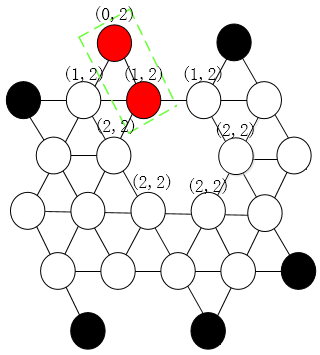
\includegraphics[width=3cm,height=3cm]{chapter3/figure3-7a.png}}
	\hspace{1cm}
	\subfigure[]{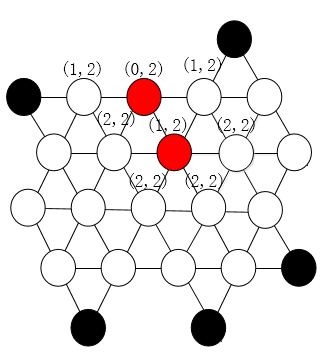
\includegraphics[width=3cm,height=3cm]{chapter3/figure3-7b.png}}
	\bicaption[fig:no_update]{修复机器人梯度无法更新情况}{修复机器人梯度无法更新情况}{Fig}{The situation that repairing robots cannot update gradient.}
\end{figure*}

图\ref{fig:gradient_diffusion}描述了梯度扩散的整个过程,包含梯度更新与梯度源节点的更新。节点上方的括号内数字含义同图\ref{fig:no_update}中的含义,即表示(梯度,梯度源节点的度)。节点颜色的深浅也同样显示了梯度值的大小,颜色越深,梯度值越小,黑色节点表示梯度源节点。图\ref{fig:gradient_diffusion}(c)中,红色数字表示经历了梯度源节点的度的更新。
\begin{figure*}[!htbp]
	\centering
	\subfigure[t=0]{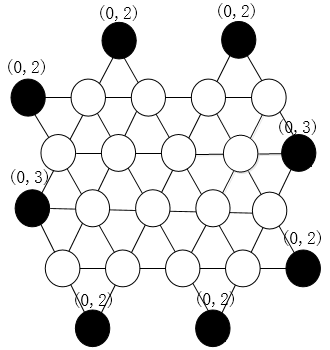
\includegraphics[width=4cm,height=4cm]{chapter3/figure3-8a.png}}
	\hspace{0.5cm}
	\subfigure[t=1]{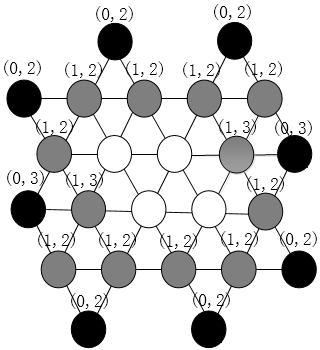
\includegraphics[width=4cm,height=4cm]{chapter3/figure3-8b.png}}
	\hspace{0.5cm}
	\subfigure[t=2]{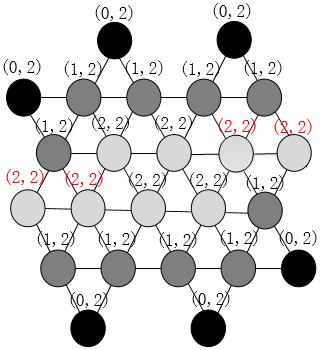
\includegraphics[width=4cm,height=4cm]{chapter3/figure3-8c.png}}
	\bicaption[fig:gradient_diffusion]{梯度扩散——梯度更新与梯度源节点的更新}{梯度扩散——梯度更新与梯度源节点的更新}{Fig}{Gradient diffusion —— gradient update and gradient source node update.}
\end{figure*}
由上述梯度扩散过程及图\ref{fig:gradient_diffusion}可的如下结论:

\begin{cor}
	\label{cor:sourcegradient_leastdegree}
	当多机器人编队网络形成稳定的梯度分布之后,编队中所有机器人梯度源节点的度都相同且等于编队中全局度最小机器人的度。
\end{cor}

\begin{cor}
	\label{cor:neighbor_gradient}
	当编队网络形成稳定的梯度分布之后,除梯度源节点外,其他机器人邻居中一定含有梯度值小于自身梯度值的机器人。
\end{cor}

\subsection{候选修复状态}
在编队中形成稳定的梯度分布之后,如果出现机器人缺失,则缺失机器人的邻居检测到缺失后会由当前的梯度源节点状态或者非梯度源节点状态转移到候选修复状态,称处于候选修复状态下的机器人为候选修复机器人。候选修复机器人会与其它候选修复机器人进行比较以确定最终的修复机器人。但是由于本文算法是完全分布式实现,机器人只能与其邻居直接通信,因此缺失机器人的邻居之间可能无法直接进行通信,如图\ref{fig:no_update}(a)所示,缺失机器人周围的邻居都会处于候选修复状态,但是如何能在其中选择出一个最佳的修复机器人呢?为解决这一问题,本文采用竞选机制。如果候选修复机器人竞选成功,则由候选修复状态转移到修复状态,如果竞选失败,则由候选修复状态转移回原状态。

\subsubsection{竞选机制}
候选修复机器人没有办法实现任意两两机器人之间的通信,所以每个机器人没有办法一次性获得所有其他候选修复机器人的信息。然而,处于候选修复状态下的机器人相互通信的目的就是要选择出最佳的修复机器人。因此,候选修复机器人没有必要同时获取到其他所有的候选修复机器人的信息,而只要能够得到所有候选修复机器人中最佳修复机器人信息即可。然后通过判断最佳修复机器人是否是自己即可最终确定出唯一的修复机器人。
\begin{defn}
	最佳修复机器人$R_b$为所有处于候选修复状态的机器人之中梯度值最小的修复机器人,即满足:
	\[
		\forall R_i \in N_e(R_f), R_b.Gra \leq R_i.Gra
	\]
\end{defn}
这里仅比较候选修复机器人的梯度值是因为在梯度源节点状态与非梯度源节点状态下编队形成稳定梯度分布之后,所有机器人的梯度源节点的度值相同。

具体竞选机制如下:\\
\indent 1).每个候选修复机器人保存一个当前最佳修复机器人信息$M$,此信息中包含机器人的编号($id$)以及梯度值($Gra$),并在初始时刻将此信息设置为自身的编号和梯度值,同时开启一个计时器$T$。\\
\indent 2).每个机器人将自身保存的最佳修复机器人信息发送给邻居。\\
\indent 3).候选修复机器人如果接收到邻居传来的最佳修复机器人信息$M_r$,则将自身的最佳修复机器人信息与其进行比较,如比较结果满足:
\[
	(M_r.Gra < M.Gra)\ ||\ (M_r.Gra == M.Gra\ \&\& \  M_r.id < M.id) 
\]
则将自身保存的最佳修复机器人信息更新为接收到的信息。\\
\indent 4).重复执行步骤2,3,4直到定时器达到最大竞选时间$T_{max}$。如果此时保存的最佳修复机器人信息中的$id$等于自身$id$,则自己为最终的修复机器人,状态转移到修复状态,否则状态转移回候选修复状态之前的状态。

算法\ref{algorithm:campaign_initial}和\ref{algorithm:campaign}是竞选机制的伪代码,其中算法\ref{algorithm:campaign_initial}是竞选机制的初始化工作,对应竞选机制的步骤1和2。算法\ref{algorithm:campaign}对应竞选机制的步骤3和4。代码中函数$SendToNeighbor(M)$并未给出具体实现,此函数功能是将信息$M$发送给邻居,属于通信函数。
\begin{algorithm}
	\caption{竞选机制初始化}
	\label{algorithm:campaign_initial}
	\begin{algorithmic}[1]
		\Require $M \leftarrow$ 自身保存的最佳修复机器人信息, $T \leftarrow$ 定时器,单位时间表示邻居间一次通信时间
		\Ensure $M \leftarrow$ 自身保存的最佳修复机器人信息, $T \leftarrow$ 定时器,单位时间表示邻居间一次通信时间
		\Function{CampaignInitial}{$M, T$}
			\State $M.Gra \gets Gra$
			\State $M.id \gets id$
			\State $T \gets 0$
			\State $SendToNeighbor(M)$
			\State \Return{$M,T$}
		\EndFunction
	\end{algorithmic}	
\end{algorithm}

\begin{algorithm}
	\caption{竞选机制}
	\label{algorithm:campaign}
	\begin{algorithmic}[1]
		\Require $M_r \leftarrow$ 邻居机器人发来的最佳修复机器人的信息
		\Ensure $IsRepairingRobot \leftarrow$ 是否为修复机器人,$true \leftarrow $是, $ false \leftarrow$ 不是
		\Function {CampaignForRepairingRobot}{$M_r$}
			\State $T \gets T+1$				
			\If {$T < T_{max}$}
				\If {$M_r.Gra < M.Gra$}
				\State $M.Gra \gets M_r.Gra$
				\State $M.id \gets M_r.id$		
			\Else 
				\If {$M_r.Gra == M.Gra \  \&\& \  M_r.id < M.id$}
%			\algstore{CampaignForRepairingRobot}
%	\end{algorithmic}
%\end{algorithm}
%\begin{algorithm}
%	\begin{algorithmic}[1]
%		\algrestore{CampaignForRepairingRobot}
						\State $M.Gra \gets M_r.Gra$
						\State $M.id \gets M.id$
					\EndIf
				\EndIf
				\State $SendToNeighbor(M)$
			\Else 
				\If {$M.id == id$}
					\State $IsRepairingRobot \gets true$
					\State \Return {$IsRepairingRobot$} 
				\EndIf	
			\EndIf			
		\EndFunction		
	\end{algorithmic}
\end{algorithm}

图\ref{fig:campaign}展示了候选修复机器人之间的竞选过程。黄色节点代表机器人处于候选修复状态,红色节点表示机器人处于修复状态。节点内部的数字表示机器人的编号$id$,节点上方的数据对表示竞选过程中邻居间传递的信息,包含梯度值和机器人编号$(Gra,id)$,其中红色数据对表示最佳修复机器人的信息。从图中可以看出经过3倍的邻居通信时间,所有候选修复机器人保存的最佳修复机器人都相同,且最佳修复机器人的$id = 12$,因此$12$号机器人竞选成功,状态转移到修复状态,其他机器人转移回原状态。
\begin{figure*}[!htbp]
	\centering
	\subfigure[$T=0$]{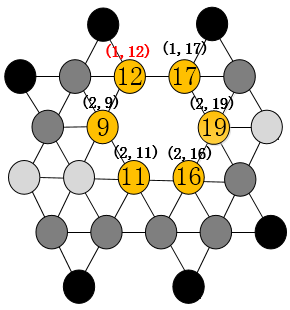
\includegraphics[width=3.5cm,height=3.5cm]{chapter3/figure3-9a.png}}
	\subfigure[$T=1$]{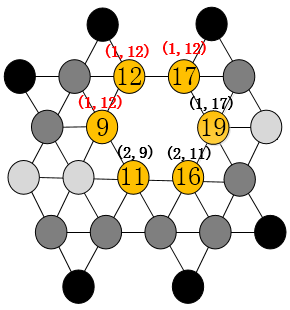
\includegraphics[width=3.5cm,height=3.5cm]{chapter3/figure3-9b.png}}
	\subfigure[$T=2$]{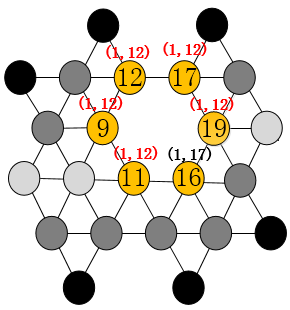
\includegraphics[width=3.5cm,height=3.5cm]{chapter3/figure3-9c.png}}
	\subfigure[$T=3=T_{max}$]{\includegraphics[width=3.5cm,height=3.5cm]{chapter3/figure3-9d.png}}
	\bicaption[fig:campaign]{候选修复机器人竞选过程}{候选修复机器人竞选过程}{Fig}{The campaign process of repairing robots candidates.}
\end{figure*}

\subsubsection{竞选时间}
\begin{lem}
	\label{lem:negotiation_time}
	最大竞选时间$T_{max}$的选择与候选修复机器人的个数$d_f$和邻居之间的通信时间$t_c$有关,满足:
	\[
		T_{max} > d_f t_c/2
	\]
	
	引理\ref{lem:negotiation_time}的证明。
	
	\begin{proof}
		当出现机器人缺失时,最坏情况下所有候选修复状态的机器人形成一个环形,若在六邻居网络中则如图\ref{fig:campaign}所示。根据上述竞选机制可知,最终$id=12$的机器人被选为修复机器人。在到达最大竞选时间之后,所有候选修复机器人记录的最佳修复机器人都为$id=12$的机器人,因此最终的修复机器人信息是从$id=12$的机器人向其他机器人传播。其中$id=16$的机器人距离$id=12$的机器人最远,信息传播时间需要$d_f t_c/2$,而其他机器人接收到信息的时间都要小于$d_f t_c/2$。因此最大竞选时间需满足:$T_{max} > d_f t_c/2$。
	\end{proof}
\end{lem}

\subsection{修复状态}

\subsubsection{修复状态传递}
当编队中出现机器人缺失时,为实现同步性改善全局最优,需要利用编队中度最小的机器人修复缺失机器人。由前文分析可知,一条修复路径终止于全局度最小机器人。因此候选修复机器人通过竞选确定了修复路径中的第一个修复机器人之后,若此修复机器人不是全局度最小机器人,则应该继续在其邻居中选择修复机器人直到全局度最小机器人,从而形成一条修复路径。由修复状态下的机器人继续选择修复机器人的过程称为修复状态传递。被选中的机器人由当前状态转移到修复状态。处于修复状态的机器人在其邻居中选择下一步的修复机器人的规则如下:\\
\indent a)选择邻居中梯度值最小的机器人最为下一步修复机器人。\\
\indent b)若邻居中存在多个梯度值最小的机器人,则选择$id$最小的机器人作为修复机器人。\\
\indent c)重复步骤a),b)直到度最小机器人为止。

修复状态下修复传递算法的伪码如下:\\
\begin{algorithm}
	\caption{修复状态传递算法}
	\label{algorithm:repairing_status_deliever}
	\begin{algorithmic}[1]
		\Require $Neighbor[] \leftarrow$ 邻居列表, $len \leftarrow$ 列表长度
		\Ensure $NextRepairingRobot \leftarrow$ 下一步修复机器人
		\Function{TransmitRepairingStatus}{$Neighbor[], len$}
			\State $NextRepairingRobot \gets Neighbor[0]$
			\State $i \gets 0$
			\While {$i < len$}
				\If {$Neighbor[i].Gra < NextRepairingRobot.Gra$}
					\State $NextRepairingRobot \gets Neighbor[i]$
				\Else
					\If {$Neighbor[i].Gra = NextRepairingRobot.Gra \ \&\& 
						\ Neighbor[i].id < NextRepairingRobot.id$}
						\State $NextRepairingRobot \gets Neighbor[i]$
					\EndIf
				\EndIf
				\State $i \gets i+1$
			\EndWhile
%					\algstore{TransmitRepairingStatus}
%	\end{algorithmic}
%\end{algorithm}
%\begin{algorithm}
%	\begin{algorithmic}
%				\algrestore{TransmitRepairingStatus}
			\State \Return{$NextRepairingRobot$}
		\EndFunction			
	\end{algorithmic}	
\end{algorithm}
	
\subsubsection{修复运动}
修复状态下的机器人,当其在邻居中选出下一步修复机器人,并将修复信息传递给下一步修复机器人之后便开始运动。由候选修复状态转移到修复状态的机器人填补缺失机器人,由梯度源节点状态或者非梯度源节点状态转移到修复状态的机器人填补上一步修复机器人留下的空缺位置。当修复机器人运动到目标位置后则由修复状态转移到梯度源节点状态或者非梯度源节点状态。

图\ref{fig:repairing_status}展示了修复状态的机器人的行为。图\ref{fig:repairing_status}(a)中修复机器人根据修复机器人选取规则进行下一步修复机器人的选择。将修复信息传递给下一步修复机器人,邻居中的10号机器人接收到修复信息后由梯度源节点状态转移到修复状态,如图\ref{fig:repairing_status}(b)所示。12号修复机器人在指定完下一步修复机器人后即向缺失机器人的位置开始运动,随后12号修复机器人也开始运动,如图\ref{fig:repairing_status}(c)所示。最终,修复机器人运动到目标位置,修复完成状态由修复状态转移到梯度源节点状态或者非梯度源节点状态。

\begin{figure*}[!htbp]
	\centering
	\subfigure[]{\includegraphics[width=3.5cm,height=3.5cm]{chapter3/figure3-10a.png}}
	\subfigure[]{\includegraphics[width=3.5cm,height=3.5cm]{chapter3/figure3-10b.png}}
	\subfigure[]{\includegraphics[width=3.5cm,height=3.5cm]{chapter3/figure3-10c.png}}
	\subfigure[]{\includegraphics[width=3.5cm,height=3.5cm]{chapter3/figure3-10d.png}}
	\bicaption[fig:repairing_status]{修复状态——修复状态传递与修复运动}{修复状态——修复状态传递与修复运动}{Fig}{RepairingStatus——the transmission of repairing status and repairing movement.}
		
\end{figure*}

\section{算法分析}

\subsection{同步性分析}
本文自修复算法的主要目的就是提高编队在机器人缺失后的运动同步性。前文已经指出编队拓扑邻接矩阵的第二大特征值$\lambda_2$可以用来衡量编队的同步性好坏。根据引理\ref{lem:degree_syn},需要用编队中全局度最小的机器人修复缺失机器人才会使得同步性改善全局最优。根据本文自修复算法,对于编队同步性的改善情况可提出以下引理。
\begin{lem}
	\label{lem:syn_analysis}
	当机器人编队网络中出现机器人缺失时,本文算法可以在编队中选出的修复机器人序列中最后一个修复机器人是全局度最小机器人。修复完成后等效成全局度最小机器人修复缺失机器人,以使得同步性改善全局最优。
	
	引理\ref{lem:syn_analysis}的证明。
	
	\begin{proof}
		采用反证法证明。假设编队中出现机器人缺失后,应用本文算法选出的修复机器人序列为$\{R_1,R_2,\dots,R_k\}$。若序列中的最后一步修复机器人$R_k$不是全局度最小的机器人,则$R_k$的梯度值$R_k.Deg > 0$。根据推论\ref{cor:neighbor_gradient}可知,在机器人$R_k$的邻居中仍然存在梯度值小于自身的机器人。由竞选机制中的修复机器人选取规则可知,此机器人会继续在邻居中选择下一步修复机器人,因此$R_k$不是修复机器人序列的最后一步修复机器人。与假设矛盾,所以假设不成立。所以当机器人编队网络中出现机器人缺失时,本文算法可以在编队中选出的修复机器人序列中最后一个修复机器人是全局度最小机器人。修复完成后等效成全局度最小机器人修复缺失机器人,以使得同步性改善全局最优。
	\end{proof}	
\end{lem}

\subsection{修复路径分析}
使得编队同步性改善达到全局最优是本文算法的目标。但是算法执行的效率也是考量算法优劣的重要指标。其中修复路径的长度是影响效率的一个重要因素。在文献\parencite{张飞2008移动机器人覆盖问题的研究}中的随机自修复算法,由于存在过大的随机性,导致最终的修复路径长短不一,随机性很大。因此,算法效率不高。分析随机自修复算法效率不高的原因可以发现,算法不能保证每一步修复机器人的选择都是有效接近度最小机器人的操作。若用梯度的概念来衡量即是每一步的选择不能保证是沿着梯度下降的方向。所以做了很多无用功。文献\parencite{liu2015gradient}中虽然引入了梯度,但是由于梯度分布的原因,无法保证每一条修复路径的选取都能达到同步性改善全局最优,即容易产生局部极小的问题。本文算法在引入梯度的基础上,采用新的梯度扩散机制,使得最终能够实现同步性改善全局最优,且在此基础上实现修复路径最短。因此,给出以下引理。
\begin{lem}
	\label{lem:repairingPath_analysis}
	在编队形成稳定梯度分布的条件下,本文算法可以找到一条最短的实现同步性改善全局最优的修复路径。
	
	引理\ref{lem:repairingPath_analysis}的证明。
	
	\begin{proof}
		利用归纳法证明。如果梯度源节点为缺失机器人,则不需要修复,修复路径长度为$0$。因此满足引理\ref{lem:repairingPath_analysis}。假设编队中某个机器人缺失后本文算法选择的一条修复路径的修复机器人序列为$\{R_1,R_2,\dots,R_k \}$,且序列中$\{R_1,R_2,\dots,R_{k-1} \}$是从$R_1$到$R_{k-1}$的一条最短路径。接下来证明从$R_1$到$R_k$的路径最短。根据假设,机器人$R_{k-1}$不是梯度源节点,又由推论\ref{cor:neighbor_gradient}可知,在其邻居中至少存在一个梯度值小于$R_{k-1}.Deg$的机器人。又由修复状态下选取下一步修复机器人规则可知,修复机器人在邻居中选择梯度值最小的机器人作为下一步修复机器人,因此机器人$R_k$为机器人$R_{k-1}$邻居中与其梯度差最大的机器人。因此$R_1$到$R_k$的路径最短。
		
		综上所述,在编队形成稳定梯度分布的条件下,本文算法可以找到一条最短的实现同步性改善全局最优的修复路径。
	\end{proof}
\end{lem}

\subsection{修复时间分析}
修复时间$t_r$是指从编队中出现机器人缺失到修复完成的时间。根据文献\parencite{张飞2008移动机器人覆盖问题的研究},对于递归自修复过程,修复时间$t_r$可定义为:
\begin{equation}
	t_r = t_d + t_m = \sum_{i+1}^k t_{di} + t_m = t_{d1} + (k-1)t_{dk} + t_m
\end{equation}
式中,\\
\indent $t_d$ —— 选择时间,选择修复机器人所花费的时间和。\\
\indent $t_m$ —— 运动时间,修复机器人移动到目标位置所需的时间。\\
\indent $t_{di}$ —— 第$i$步修复机器人的选择时间。

假设在一条修复路径中存在4个修复机器人,则这4个修复机器人的修复时间示意图如图\ref{fig:repairing_time}所示。
\begin{figure}[!htbp]
	\centering
	\includegraphics[width=8cm,height=4cm]{chapter3/figure3-11.png}
	\bicaption[fig:repairing_time]{修复时间示意图}{修复时间示意图}{Fig}{Diagram of the repairing time.}
\end{figure}
$t_{d1}$为竞选时间,$t_{m_1}$为竞选成功的第一步修复机器人运动到缺失机器人位置的运动时间。$t_{d2}~t_{d4}$分别为处于修复状态的机器人在选择下一步修复机器人的选择时间和消息传递时间之和。$t_{m2}~t_{m4}$为被选中的后续修复机器人在填补上一步修复机器人留下的空缺时的运动时间。为简化问题描述,则假设编队中机器人与邻居之间的距离都相等。所以运动时间$t_{m1} = t_{m2} = t_{m3} = t_{m4}$。有因为修复机器人$t_2 ~ t_4$都是由上一步修复机器人在邻居中根据相同的选取规则指定的,所以选择时间$t_{d2} = t_{d3} = t_{d4}$。而$t_{d1}$为竞选时间,需要更多的机器人参与信息决策与消息传递,因此$t_{d1} > t_{d2} = t_{d3} = t_{d4}$。又因为在本文算法自修复过程中,每一个修复机器人通知完下一步修复机器人即开始运动,因此总的修复时间即为$t_r$。总的修复时间中只包含一倍的运动时间,而相比选择时间,运动时间占据总的修复时间比例要大得多。因此本文算法在修复时间上更具优势。

\section{本章小结}
本章主要就多机器人编队中出现机器人缺失导致同步性下降的问题提出了一种同步性改善全局最优的递归自修复算法。在分析了早期工作,对比编队中有无梯度信息的差别之后,本文引入梯度信息。并通过改进梯度扩散的方式之后,使得同步性改善达到全局最优。利用有限状态机的方式主要通过5种状态描述本文自修复算法,包括初始状态,梯度源节点状态,非梯度源节点状态,候选修复状态和修复状态。针对每一种状态下算法的执行过程给出了详细的分析和介绍。最后从同步性,修复路径,修复时间等几个方面分析了本文算法的优势。总结起来,本章主要贡献如下:\\
\indent 1)提出了新的梯度扩散过程,在梯度扩散过程中,邻居间传递的信息不仅包括梯度信息,还包括梯度源节点的度的信息,从而可以避免局部极小的问题。\\
\indent 2)利用状态机描述算法,方便算法的实现与机器人的控制。\\
\indent 3)对于所有候选修复下的机器人无法直接通信问题,提出了竞选机制,使得在保证完全分布式控制的条件下实现候选修复状态下的修复机器人的选取。\\
\indent 4)从多个指标分析了本文算法的性能。

\chapter{自修复实验系统设计}
为验证本文算法的有效性和可行性。本章设计了一套切实可行的试验系统,并在改系统下成功进行了同步性改善全局最优自修复实验。

\section{系统需求}
在设计系统之前需要明确系统都需要哪些功能。根据前文对自修复算法的描述和分析可知,首先需要有多个机器人实体来完成编队控制和算法执行。实验中为使得多机器人能够保持编队并顺利执行修复动作,机器人必须知道自身的位置,以及邻居机器人的位置信息。因此该系统需要获取机器人的位置信息。当编队中机器人出现缺失时,其邻居机器人要能够判断出邻居的丢失。在梯度扩散与修复状态传递的过程中还需要编队机器人内部的信息通信。另外对于系统的运行与停止需要我们人为的控制,而多个机器人无法手动同时开启或停止,所以需要设计一个远程控制平台来对整个编队进行控制,同时还能够检测编队中各个机器人的转态。本章实验系统主要围绕以上功能需求而设计。

\section{系统框架及组成}
根据以上需求可知,本实验系统主要具备3大功能部分:定位系统、机器人个体控制及通信系统、远程控制系统。图\ref{fig:system_structure}描述了整个系统的框架图,下面依次介绍3个子系统的设计。
\begin{figure}[!htbp]
	\centering
	\includegraphics[width=10cm,height=8cm]{chapter4/figure4-3.png}
	\bicaption[fig:system_structure]{试验系统框架示意图}{试验系统框架示意图}{Fig}{The schematic diagram of experimental system.}
\end{figure}

\subsection{定位系统}
本实验系统的定位系统主要采用Vicon光学运动捕捉系统进行机器人的空间定位。Vicon光学运动捕捉系统是由世界上一家非常著名的光学动作捕捉(Motion Capture)系统供应商英国Oxford Metrics Limited 公司生产。它的这项技术在70年代服务于英国海军,从事遥感、测控技术设备的研究与生产。进入80年代他们将自己在军事领域里的高新技术逐渐用于民用方面,在医疗、运动、工程、生物等诸多领域生产制造用于运动捕捉的Motion Capture系统。80年代末,OML公司又将动作捕捉系统技术应用于影视的动画制作领域。
\begin{figure}[!htbp]
	\centering
	\subfigure[运动捕捉系统]{\includegraphics[width=8cm,height=6cm]{chapter4/figure4-1a.png}}
	\subfigure[Vicon 摄像头]{\includegraphics[width=5cm,height=4cm]{chapter4/figure4-1b.jpg}}
	\bicaption[fig:vicon_camera]{Vicon光学运动捕捉系统示意图}{Vicon光学运动捕捉系统}{Fig}{The Vicon motion capture system.}
\end{figure}

Vicon 是英国 OML 公司生产的光学动作捕捉 motion capture 系统。它是世界上第一个设计用于运动捕捉的光学系统,它以自己非凡的技术性能在 motion capture 系统硬件制造领域赢得了极高的声誉,并且改写了 motion capture 系统传统意义上涵盖的内容。它由一组网络连接的 Vicon MX 运动捕捉摄像机和其它设备,建立起一个完整的三维运动捕获系统,以提供实时光学数据,这些数据可以被应用于实时在线或者离线的运动捕捉、分析,应用领域涉及动画制作、虚拟现实系统、机器人遥控、互动式游戏、体育训练、人体工程学研究、生物力学研究等方面。

Vicon运动捕捉系统的主要功能为:

Vicon 系统是非常准确和可靠的光学动作捕捉系统,它所提供的实时光学数据,可以被应用于实时在线或者离线的运动捕捉、分析。

特点:\\
\indent 1)Vicon 公司开发了自己专利的 Vicon Vegas 传感器,可以实现高分辨率与高捕捉频率的同时性,实时捕捉三维效果好,功能强。\\
\indent 2)MX Control 提供 Vicon MX 系统与第三方设备之间的接口,包括测力板、肌电设备、音频、数据手套、眼球跟踪器或者其它数字设备,也可以包含其它附加的板卡以增强 Vicon MX 系统的功能。\\
\indent 3)捕捉摄像机精度高,得到数据非常稳定,捕捉距离也更远。\\
\indent 4)局部捕捉标记点即使被身体挡住,经过软件处理后仍然可以得到令人满意的输出数据。\\
\indent 5)MX 系统安装、调试方便,脱离了旧系统的数据服务器,运输携带更方便。\\
\indent 6)软件界面人性化,数据处理能力强,批处理功能十分方便。

如此高性能的运动捕捉设备,配合Vicon的应用软件Tracker3可以实现高精度,低延迟,多目标的机器人空间定位系统。结合Tracker3应用软件,系统具有如下性能特点:\\
\indent 1)摄像头越多可追踪目标数越多。最低延迟可达到2.8ms处理10个目标,1.9ms处理5个目标。\\
\indent 2)数据从观测端到使用端5ms低延迟。\\
\indent 3)集成实时数据引擎,可以为第三方应用提供数据流,并支持单播TCP链接和多播UDP链接。\\
\indent 4)结合Vicon DataStream SDK 接口,支持 C++, .NET, Windows, Linux, ROS等,方便开发。\\
\indent 5)记录原始数据,支持回放以及离线数据分析。

为使如此高性能的设备充分发挥价值,在定位系统设计时就需要考虑开发的可扩展性,以及功能的丰富性。

\subsection{机器人个体控制及通信系统}
本实验系统机器人个体采用本实验室自主研发的Frontier \uppercase\expandafter{\romannumeral3} 型自主移动机器人平台,如图\ref{fig:robot_zigbee}(a)所示。小车上搭载ASUS Eee PC 900HA笔记本电脑作为控制中心,分布式自修复算法运行在此笔记本之上。笔记本通过串口向小车的运动控制器发送速度信息从而控制小车运动。小车上安装有反光球用于运动捕捉系统的识别与定位。
\begin{figure*}[!htbp]
	\centering
	\subfigure[机器人个体]{\includegraphics[width=5cm,height=4cm]{chapter4/figure4-2a.png}}
	\hspace{1cm}
	\subfigure[ZigBee通信模块]{\includegraphics[width=5cm,height=4cm]{chapter4/figure4-2b.png}}
	\bicaption[fig:robot_zigbee]{机器人个体与ZigBee通信模块}{机器人个体与ZigBee通信模块}{Fig}{The robot and ZigBee communication model.}
\end{figure*}

在本系统中包含有多种方向的通信,包括定位系统与机器人之间的通信,远程控制系统与机器人之间的通信,机器人与机器人之间的通信。其中,定位系统与机器人之间的通信采用局域网内部的网络通信方式。而机器人之间的通信由于需要多对多通信,且通信频繁数据量小,再有通信拓扑在算法执行过程中会动态建立以及切换,所以采用ZigBee作为机器人之间的组网通信方式,如图\ref{fig:robot_zigbee}(b)所示。ZigBee通信网络具有低功耗、低成本、近距离、短时延、高安全、工作频段灵活等特性。另外,主要是ZigBee的自组网通信方式可以轻松满足K邻居拓扑网络的构建与拓扑切换的需求。

\subsection{远程控制系统}
远程控制系统主要是为实现对编队机器人同时控制,且显示各个机器人状态信息。远程控制的实现主要通过ZigBee网络中的协调器对所有编队机器人进行广播。

\section{系统设计}

\subsection{定位系统}
鉴于Vicon光学运动捕捉系统的强大功能,本系统的设计不只考虑用于多机器人编队自修复的定位需求,同时考虑本实验室的多种机器人如无人机、机械臂,软体手术机器人的空间定位需求而开发。另外在设计过程中充分考虑了功能的可扩展性,方便以后机器人种类的增加或者功能的变化。在几种机器人当中根据结构可以大致分为两类,一种是刚体机器人,如本实验所需的小车,无人机,机械臂。另一种是柔性机器人,如软体手术机器人。针对这两类需求,Vicon运动捕捉系统提供了两款应用软件Tracker和Nexus。在这两款软件上可以对Vicon摄像头进行命名、参数配置和调整、标定、目标选择与命名等操作。然而这两款软件无法满足某些特定应用场景的需求,因此本文介绍的系统是在Vicon官方开放的sdk基础上进行的二次开发以满足本实验系统以及其他特定种类机器人的需求。本文定位系统设计的主要工作是开发了一款服务器端软件,软件集成了空间机器人的数据采集,分析,封装,转发,显示,存储等功能。开发环境为\textbf{Windows7}操作系统下的\textbf{visual studio 2013}编辑器,采用\textbf{MFC}框架。

对于刚体结构的机器人和柔性结构的机器人Tracker和Nexus提供的数据形式不同,因此针对两类需求分别设计了不同的数据处理方式以及UI显示界面。在程序启动时需要根据具体需求选择不同的应用模式,如图\ref{fig:select_mode}所示,软件分为ViconSystem\_Nexus模式和ViconSystem\_Tracker模式,分别针对Nexus软件和Tracker软件使用。
\begin{figure}[!htbp]
	\centering
	\includegraphics[width=8cm,height=5.5cm]{chapter4/figure4-4.png}
	\bicaption[fig:select_mode]{软件模式选择}{软件模式选择}{Fig}{Selection of software mode.}
\end{figure}

目前,由于ViconSystem\_Nexus模式下除软件的数据处理方式与部分UI界面与ViconSystem\_Tracker不同外其他功能类似,且数据种类不如ViconSystem\_Tracker模式下丰富。因此下文主要根据ViconSystem\_Tracker模式的软件开发进行介绍。

图\ref{fig:software_diagram}描述了定位系统的软件结构层次。不同层对应系统不同部分。
\begin{figure}[!htbp]
	\centering
	\includegraphics[width=4cm,height=6cm]{chapter4/figure4-5.png}
	\bicaption[fig:software_diagram]{软件结构层次图}{软件结构层次图}{Fig}{Software structure level diagram.}	
\end{figure}

\indent \textbf{硬件驱动层与数据采集层:}这两层对应Vicon运动捕捉系统的硬件设施与Tracker应用软件。Vicon系统服务器驱动10台运动捕捉相机,对相机进行标定之后,在Tracker软件中根据识别的反光球标记机器人并命名。运动捕捉相机将采集的数据上传到数据中心,在数据中心中对相机数据进行处理,计算出空间中各个机器人的位姿信息。\\
\indent \textbf{数据处理层与通信层:}本文所开发的软件主要是属于这两层。软件通过sdk提供的接口将数据中心计算的位姿信息获取到,然后进一步对数据进行处理,显示、存储、以及封装成应用层需要的数据形式。在通信层将封装好的数据通过局域网内的wifi传输给应用层。\\
\indent \textbf{应用层:}这一层主要对应机器人,如何使用数据取决于机器人要实现的功能。

图\ref{fig:flow_chart}是程序设计的流程图,程序采用多线程设计,主要分为数据采集与处理线程和数据传输线程,在两个线程之间存在数据同步。
\begin{figure}[!htbp]
	\centering
	\includegraphics[width=8cm,height=7cm]{chapter4/FlowChart.png}
	\bicaption[fig:flow_chart]{定位系统程序设计流程图}{定位系统程序设计流程图}{Fig}{The program flow chart of positioning system software.}
\end{figure}

图\ref{fig:software_ui}是软件的用户界面。
\begin{figure}[!htbp]
	\centering
	\includegraphics[width=10cm,height=8cm]{chapter4/figure4-6.png}
	\bicaption[fig:software_ui]{定位系统ViconSystem\_Tracker模式软件界面}{定位系统ViconSystem\_Tracker模式软件界面}{Fig}{The user interface of ViconSystem\_Tracker mode.}
\end{figure}

软件实现的主要功能有:\\
\indent 1)实现目标在空间中的位置、旋转矢量、旋转矩阵、四元数、欧拉角等数据的实时采集与显示。\\
\indent 2)支持多客户端链接,并实时发送以上数据到客户端,发送的数据可以按照需求在数据选择框中进行勾选。\\
\indent 3)数据发送方式支持TCP协议和UDP协议。\\
\indent 4)支持发送周期可调(单位ms),系统初始默认周期为100ms。\\
\indent 5)支持数据本地存储,方便离线分析。数据存储的类型与发送给客户端的数据类型同步,都是根据在数据选择框中所勾选的数据进行处理。数据本地记录的周期可调,默认为10ms。

ViconSystem\_Tracker模式主要是针对刚体在空间中的位姿数据获取,每一个刚体需要贴3个以上的反光球。获取到的数据是整个刚体的位姿数据。例如空间位置是刚体上所有反光球位置的平均值。但是考虑柔性结构的机器人,它在空间中会发生形变,因此我们想要得到的数据是柔性结构的每一点的位置数据。ViconSystem\_Nexus即是为此需求而设计,背后依托的是Vicon运动捕捉系统的Nexus软件。在ViconSystem\_Nexus下没有各种不同的位姿数据,只显示每个反光球在空间中的位置数据。其他功能与ViconSystem\_Tracker模式下类似,因此不再具体介绍。软件用户界面如图\ref{fig:software_ui2}所示。
\begin{figure}[!htbp]
	\centering
	\includegraphics[width=10cm,height=8cm]{chapter4/figure4-7.png}
	\bicaption[fig:software_ui2]{定位系统ViconSystem\_Nexus模式软件界面}{定位系统ViconSystem\_Nexus模式软件界面}{Fig}{The user interface of ViconSystem\_Nexus mode.}
\end{figure}

\subsection{机器人个体与通信系统}
机器人个体控制主要是在ASUS Eee PC 900HA笔记本电脑上实现第3章所描述的自修复算法,开发环境为vc6.0。通过串口向基于DSP实现的运动控制板发送速度命令。利用ZigBee与邻居进行通信,同时通过ZigBee与远程控制端进行交互。图\ref{fig:clientSoftware}是机器人个体控制的用户界面,继承了参数设置,状态显示,运动控制的功能。

\begin{figure}[!htbp]
	\centering
	\includegraphics[width=10cm,height=6cm]{chapter4/figure4-8.png}
	\bicaption[fig:clientSoftware]{机器人个体控制的软件用户界面}{机器人个体控制的软件用户界面}{Fig}{The user interface of robot client software.}
\end{figure}

\subsection{远程控制系统}
远程控制系统主要是通过串口连接ZigBee网络的协调器,利用协调器向编队网络发送运动控制指令以及少量数据,同时接受来自所有机器人的状态信息并显示,图\ref{fig:RopSoftware}是远程控制端的用户界面。

\begin{figure}[!htbp]
	\centering
	\includegraphics[width=10cm,height=6cm]{chapter4/figure4-9.png}
	\bicaption[fig:RopSoftware]{远程控制系统软件用户界面}{远程控制系统软件用户界面}{Fig}{The user interface of romote operation software.}
\end{figure}

\section{本章小结}
本章介绍了多机器人编队自修复实验平台的设计。实验平台主要包括定位系统,机器人个体控制与通信系统,远程控制系统。其中着重介绍了定位系统的设计,依托Vicon光学运动捕捉系统,设计了功能丰富,适用不同机器人,可扩展的定位系统服务器端软件。机器人个体与通信系统实现了本文的同步性改善全局最优的分布式递归自修复算法。远程控制系统实现对编队的远程统一控制与转态回显。

\chapter{自修复实验系统设计}
为验证本文算法的有效性和可行性。本章设计了一套切实可行的试验系统,并在该系统下成功进行了同步性改善全局最优自修复实验。

%\section{自修复实验系统}
\section{系统需求}
在设计系统之前需要明确系统都需要哪些功能。根据前文对自修复算法的描述和分析可知,首先需要有多个机器人实体来完成编队控制和算法执行。实验中为使得多机器人能够保持编队并顺利执行修复动作,机器人必须知道自身的位置,以及邻居机器人的位置信息。因此该系统需要获取机器人的位置信息。当编队中机器人出现缺失时,其邻居机器人要能够判断出邻居的丢失。在梯度扩散与修复状态传递的过程中还需要编队机器人内部的信息通信。另外对于系统的运行与停止需要我们人为的控制,而多个机器人无法手动同时开启或停止,所以需要设计一个远程控制平台来对整个编队进行控制,同时还能够检测编队中各个机器人的转态。本章实验系统主要围绕以上功能需求而设计。

\section{系统框架及组成}
根据以上需求可知,本实验系统主要具备3大功能部分:定位系统、机器人个体控制及通信系统、远程控制系统。图\ref{fig:system_structure}描述了整个系统的框架图,下面依次介绍3个子系统的设计。
\begin{figure}[!htbp]
	\centering
	\includegraphics[width=10cm,height=8cm]{chapter4/figure4-3.png}
	\bicaption[fig:system_structure]{试验系统框架示意图}{试验系统框架示意图}{Fig}{The schematic diagram of experimental system.}
\end{figure}

\subsection{定位系统}
本实验系统的定位系统主要采用Vicon光学运动捕捉系统进行机器人的空间定位。Vicon光学运动捕捉系统是由世界上一家非常著名的光学动作捕捉(Motion Capture)系统供应商英国Oxford Metrics Limited 公司生产。它的这项技术在70年代服务于英国海军,从事遥感、测控技术设备的研究与生产。进入80年代他们将自己在军事领域里的高新技术逐渐用于民用方面,在医疗、运动、工程、生物等诸多领域生产制造用于运动捕捉的Motion Capture系统。80年代末,OML公司又将动作捕捉系统技术应用于影视的动画制作领域。
\begin{figure}[!htbp]
	\centering
	\subfigure[运动捕捉系统]{\includegraphics[width=8cm,height=6cm]{chapter4/figure4-1a.png}}
	\subfigure[Vicon 摄像头]{\includegraphics[width=5cm,height=4cm]{chapter4/figure4-1b.jpg}}
	\bicaption[fig:vicon_camera]{Vicon光学运动捕捉系统示意图}{Vicon光学运动捕捉系统}{Fig}{The Vicon motion capture system.}
\end{figure}

Vicon 是英国 OML 公司生产的光学动作捕捉 motion capture 系统。它是世界上第一个设计用于运动捕捉的光学系统,它以自己非凡的技术性能在 motion capture 系统硬件制造领域赢得了极高的声誉,并且改写了 motion capture 系统传统意义上涵盖的内容。它由一组网络连接的 Vicon MX 运动捕捉摄像机和其它设备,建立起一个完整的三维运动捕获系统,以提供实时光学数据,这些数据可以被应用于实时在线或者离线的运动捕捉、分析,应用领域涉及动画制作、虚拟现实系统、机器人遥控、互动式游戏、体育训练、人体工程学研究、生物力学研究等方面。

Vicon运动捕捉系统的主要功能为:

Vicon 系统是非常准确和可靠的光学动作捕捉系统,它所提供的实时光学数据,可以被应用于实时在线或者离线的运动捕捉、分析。

特点:\\
\indent 1)Vicon 公司开发了自己专利的 Vicon Vegas 传感器,可以实现高分辨率与高捕捉频率的同时性,实时捕捉三维效果好,功能强。\\
\indent 2)MX Control 提供 Vicon MX 系统与第三方设备之间的接口,包括测力板、肌电设备、音频、数据手套、眼球跟踪器或者其它数字设备,也可以包含其它附加的板卡以增强 Vicon MX 系统的功能。\\
\indent 3)捕捉摄像机精度高,得到数据非常稳定,捕捉距离也更远。\\
\indent 4)局部捕捉标记点即使被身体挡住,经过软件处理后仍然可以得到令人满意的输出数据。\\
\indent 5)MX 系统安装、调试方便,脱离了旧系统的数据服务器,运输携带更方便。\\
\indent 6)软件界面人性化,数据处理能力强,批处理功能十分方便。

如此高性能的运动捕捉设备,配合Vicon的应用软件Tracker3可以实现高精度,低延迟,多目标的机器人空间定位系统。结合Tracker3应用软件,系统具有如下性能特点:\\
\indent 1)摄像头越多可追踪目标数越多。最低延迟可达到2.8ms处理10个目标,1.9ms处理5个目标。\\
\indent 2)数据从观测端到使用端5ms低延迟。\\
\indent 3)集成实时数据引擎,可以为第三方应用提供数据流,并支持单播TCP链接和多播UDP链接。\\
\indent 4)结合Vicon DataStream SDK 接口,支持 C++, .NET, Windows, Linux, ROS等,方便开发。\\
\indent 5)记录原始数据,支持回放以及离线数据分析。

为使如此高性能的设备充分发挥价值,在定位系统设计时就需要考虑开发的可扩展性,以及功能的丰富性。

\subsection{机器人个体控制及通信系统}
本实验系统机器人个体采用本实验室自主研发的Frontier \uppercase\expandafter{\romannumeral3} 型自主移动机器人平台,如图\ref{fig:robot_zigbee}(a)所示。小车上搭载ASUS Eee PC 900HA笔记本电脑作为控制中心,分布式自修复算法运行在此笔记本之上。笔记本通过串口向小车的运动控制器发送速度信息从而控制小车运动。小车上安装有反光球用于运动捕捉系统的识别与定位。
\begin{figure*}[!htbp]
	\centering
	\subfigure[机器人个体]{\includegraphics[width=5cm,height=4cm]{chapter4/figure4-2a.png}}
	\hspace{1cm}
	\subfigure[ZigBee通信模块]{\includegraphics[width=5cm,height=4cm]{chapter4/figure4-2b.png}}
	\bicaption[fig:robot_zigbee]{机器人个体与ZigBee通信模块}{机器人个体与ZigBee通信模块}{Fig}{The robot and ZigBee communication model.}
\end{figure*}

在本系统中包含有多种方向的通信,包括定位系统与机器人之间的通信,远程控制系统与机器人之间的通信,机器人与机器人之间的通信。其中,定位系统与机器人之间的通信采用局域网内部的网络通信方式。而机器人之间的通信由于需要多对多通信,且通信频繁数据量小,再有通信拓扑在算法执行过程中会动态建立以及切换,所以采用ZigBee作为机器人之间的组网通信方式,如图\ref{fig:robot_zigbee}(b)所示。ZigBee通信网络具有低功耗、低成本、近距离、短时延、高安全、工作频段灵活等特性。另外,主要是ZigBee的自组网通信方式可以轻松满足K邻居拓扑网络的构建与拓扑切换的需求。

\subsection{远程控制系统}
远程控制系统主要是为实现对编队机器人同时控制,且显示各个机器人状态信息。远程控制的实现主要通过ZigBee网络中的协调器对所有编队机器人进行广播。

\section{系统设计}

\subsection{定位系统}
鉴于Vicon光学运动捕捉系统的强大功能,本系统的设计不只考虑用于多机器人编队自修复的定位需求,同时考虑本实验室的多种机器人如无人机、机械臂,软体手术机器人的空间定位需求而开发。另外在设计过程中充分考虑了功能的可扩展性,方便以后机器人种类的增加或者功能的变化。在几种机器人当中根据结构可以大致分为两类,一种是刚体机器人,如本实验所需的小车,无人机,机械臂。另一种是柔性机器人,如软体手术机器人。针对这两类需求,Vicon运动捕捉系统提供了两款应用软件Tracker和Nexus。在这两款软件上可以对Vicon摄像头进行命名、参数配置和调整、标定、目标选择与命名等操作。然而这两款软件无法满足某些特定应用场景的需求,因此本文介绍的系统是在Vicon官方开放的sdk基础上进行的二次开发以满足本实验系统以及其他特定种类机器人的需求。本文定位系统设计的主要工作是开发了一款服务器端软件,软件集成了空间机器人的数据采集,分析,封装,转发,显示,存储等功能。开发环境为\textbf{Windows7}操作系统下的\textbf{visual studio 2013}编辑器,采用\textbf{MFC}框架。

对于刚体结构的机器人和柔性结构的机器人Tracker和Nexus提供的数据形式不同,因此针对两类需求分别设计了不同的数据处理方式以及UI显示界面。在程序启动时需要根据具体需求选择不同的应用模式,如图\ref{fig:select_mode}所示,软件分为ViconSystem\_Nexus模式和ViconSystem\_Tracker模式,分别针对Nexus软件和Tracker软件使用。
\begin{figure}[!htbp]
	\centering
	\includegraphics[width=8cm,height=5.5cm]{chapter4/figure4-4.png}
	\bicaption[fig:select_mode]{软件模式选择}{软件模式选择}{Fig}{Selection of software mode.}
\end{figure}

目前,由于ViconSystem\_Nexus模式下除软件的数据处理方式与部分UI界面与ViconSystem\_Tracker不同外其他功能类似,且数据种类不如ViconSystem\_Tracker模式下丰富。因此下文主要根据ViconSystem\_Tracker模式的软件开发进行介绍。

图\ref{fig:software_diagram}描述了定位系统的软件结构层次。不同层对应系统不同部分。
\begin{figure}[!htbp]
	\centering
	\includegraphics[width=4cm,height=6cm]{chapter4/figure4-5.png}
	\bicaption[fig:software_diagram]{软件结构层次图}{软件结构层次图}{Fig}{Software structure level diagram.}	
\end{figure}

\indent \textbf{硬件驱动层与数据采集层:}这两层对应Vicon运动捕捉系统的硬件设施与Tracker应用软件。Vicon系统服务器驱动10台运动捕捉相机,对相机进行标定之后,在Tracker软件中根据识别的反光球标记机器人并命名。运动捕捉相机将采集的数据上传到数据中心,在数据中心中对相机数据进行处理,计算出空间中各个机器人的位姿信息。\\
\indent \textbf{数据处理层与通信层:}本文所开发的软件主要是属于这两层。软件通过sdk提供的接口将数据中心计算的位姿信息获取到,然后进一步对数据进行处理,显示、存储、以及封装成应用层需要的数据形式。在通信层将封装好的数据通过局域网内的wifi传输给应用层。\\
\indent \textbf{应用层:}这一层主要对应机器人,如何使用数据取决于机器人要实现的功能。

图\ref{fig:flow_chart}是程序设计的流程图,程序采用多线程设计,主要分为数据采集与处理线程和数据传输线程,在两个线程之间存在数据同步。
\begin{figure}[!htbp]
	\centering
	\includegraphics[width=8cm,height=7cm]{chapter4/FlowChart.png}
	\bicaption[fig:flow_chart]{定位系统程序设计流程图}{定位系统程序设计流程图}{Fig}{The program flow chart of positioning system software.}
\end{figure}

图\ref{fig:software_ui}是软件的用户界面。
\begin{figure}[!htbp]
	\centering
	\includegraphics[width=10cm,height=8cm]{chapter4/figure4-6.png}
	\bicaption[fig:software_ui]{定位系统ViconSystem\_Tracker模式软件界面}{定位系统ViconSystem\_Tracker模式软件界面}{Fig}{The user interface of ViconSystem\_Tracker mode.}
\end{figure}

软件实现的主要功能有:\\
\indent 1)实现目标在空间中的位置、旋转矢量、旋转矩阵、四元数、欧拉角等数据的实时采集与显示。\\
\indent 2)支持多客户端链接,并实时发送以上数据到客户端,发送的数据可以按照需求在数据选择框中进行勾选。\\
\indent 3)数据发送方式支持TCP协议和UDP协议。\\
\indent 4)支持发送周期可调(单位ms),系统初始默认周期为100ms。\\
\indent 5)支持数据本地存储,方便离线分析。数据存储的类型与发送给客户端的数据类型同步,都是根据在数据选择框中所勾选的数据进行处理。数据本地记录的周期可调,默认为10ms。

ViconSystem\_Tracker模式主要是针对刚体在空间中的位姿数据获取,每一个刚体需要贴3个以上的反光球。获取到的数据是整个刚体的位姿数据。例如空间位置是刚体上所有反光球位置的平均值。但是考虑柔性结构的机器人,它在空间中会发生形变,因此我们想要得到的数据是柔性结构的每一点的位置数据。ViconSystem\_Nexus即是为此需求而设计,背后依托的是Vicon运动捕捉系统的Nexus软件。在ViconSystem\_Nexus下没有各种不同的位姿数据,只显示每个反光球在空间中的位置数据。其他功能与ViconSystem\_Tracker模式下类似,因此不再具体介绍。软件用户界面如图\ref{fig:software_ui2}所示。
\begin{figure}[!htbp]
	\centering
	\includegraphics[width=10cm,height=8cm]{chapter4/figure4-7.png}
	\bicaption[fig:software_ui2]{定位系统ViconSystem\_Nexus模式软件界面}{定位系统ViconSystem\_Nexus模式软件界面}{Fig}{The user interface of ViconSystem\_Nexus mode.}
\end{figure}

\subsection{机器人个体与通信系统}
机器人个体控制主要是在ASUS Eee PC 900HA笔记本电脑上实现第3章所描述的自修复算法,开发环境为vc6.0。通过串口向基于DSP实现的运动控制板发送速度命令。利用ZigBee与邻居进行通信,同时通过ZigBee与远程控制端进行交互。图\ref{fig:clientSoftware}是机器人个体控制的用户界面,继承了参数设置,状态显示,运动控制的功能。

\begin{figure}[!htbp]
	\centering
	\includegraphics[width=10cm,height=6cm]{chapter4/figure4-8.png}
	\bicaption[fig:clientSoftware]{机器人个体控制的软件用户界面}{机器人个体控制的软件用户界面}{Fig}{The user interface of robot client software.}
\end{figure}

\subsection{远程控制系统}
远程控制系统主要是通过串口连接ZigBee网络的协调器,利用协调器向编队网络发送运动控制指令以及少量数据,同时接受来自所有机器人的状态信息并显示,图\ref{fig:RopSoftware}是远程控制端的用户界面。

\begin{figure}[!htbp]
	\centering
	\includegraphics[width=10cm,height=6cm]{chapter4/figure4-9.png}
	\bicaption[fig:RopSoftware]{远程控制系统软件用户界面}{远程控制系统软件用户界面}{Fig}{The user interface of romote operation software.}
\end{figure}

\section{实验设计}
根据实际环境与设备条件,本实验采用6台Frontier \uppercase\expandafter{\romannumeral3}型自主移动机器人,按照6邻居网络模型编成图\ref{fig:experiment_topo}所示队形,这里将机器人进行编号以方便描述。
\begin{figure}[!htbp]
	\centering
	\includegraphics[width=6cm,height=5cm]{chapter5/figure5-12.png}
	\bicaption[fig:experiment_topo]{自修复实验编队模型}{自修复实验编队模型}{Fig}{The formation model of the self-healing experiment.}
\end{figure}
从图中可知,1号机器人是编队中度最小的机器人,因此根据梯度扩散规则1号机器人是梯度源节点,其他单个机器人的丢失都将由它来进行修复。在编队中2号和4号机器人是度局部极小机器人。若按照文献\parencite{liu2015gradient}中的梯度扩散规则,则2号和4号机器人也是梯度源节点并且无法得到更新。在实验中我们另5号机器人丢失,如果按照文献\parencite{liu2015gradient}的自修复规则,最终会由2号机器人进行修复,修复后的编队如图\ref{fig:local_experiment_result}所示。
\begin{figure}
	\centering
	\includegraphics[width=6cm,height=5cm]{chapter5/figure5-13.png}
	\bicaption[fig:local_experiment_result]{局部最优自修复算法实验结果}{局部最优自修复算法实验结果}{Fig}{The experiment result of local optimal self-healing algorithm.}
\end{figure}

\begin{figure*}[!htbp]
	\centering
	\subfigure[]{\includegraphics[width=5cm,height=4cm]{chapter5/figure5-14a.png}}
	\subfigure[]{\includegraphics[width=5cm,height=4cm]{chapter5/figure5-14b.png}}
	\subfigure[]{\includegraphics[width=5cm,height=4cm]{chapter5/figure5-14c.png}}
	\subfigure[]{\includegraphics[width=5cm,height=2.5cm]{chapter5/figure5-14d.png}}
	\bicaption[fig:global_experiment_process]{全局最优自修复算法实验过程}{全局最优自修复算法实验过程}{Fig}{The experiment process of global optimal self-healing algorithm.}
\end{figure*}

若采用本文算法,则自修复过程如图\ref{fig:global_experiment_process}所示,在5号机器人丢失后,根据竞选机制,3号机器人会竞选成功,成为第一步的修复机器人,填补5号机器人的空缺位置,5号机器人会在邻居中选取下一步的修复机器人并将修复状态传递给它。根据修复机器人选取规则,1号机器人会被选为下一步的修复机器人,填补3号机器人的空缺。1号机器人是全局度最小机器人,因此修复状态传递结束。修复完成后的编队如图\ref{fig:global_experiment_process}(d)。
\begin{figure*}[!htbp]
	\centering
	\begin{tabular}{cc}
		\subfigure[]{\includegraphics[width=8cm,height=4cm]{chapter5/figure5-15aaa.png}} & 
		\subfigure[]{\includegraphics[width=8cm,height=4cm]{chapter5/figure5-15bbb.png}} \\
		\subfigure[]{\includegraphics[width=8cm,height=4cm]{chapter5/figure5-15ccc.png}} &
		\subfigure[]{\includegraphics[width=8cm,height=4cm]{chapter5/figure5-15ddd.png}}
	\end{tabular}
	\bicaption[fig:real_experiment]{真实实验中多机器人编队的同步性改善全局最优自修复过程}{真实实验中多机器人编队的同步性改善全局最优自修复过程}{Fig}{The process of global optimal synchroniation improvement self-healing in real experiment.}
\end{figure*}
图\ref{fig:real_experiment}展示了真实实验场景及过程,图中左半部分是实际Frontier \uppercase\expandafter{\romannumeral3}型自主移动机器人组成的编队队形,右半部分是在Vicon运动捕捉系统上观测到的编队图像。实验中人为取走编队中的机器人使其失效,编队能够自主的完成预期的修复效果,多次实验均能保证修复效果,证明本文算法的实际可行性和稳定性。

\section{本章小结}
本章介绍了多机器人编队自修复实验平台的设计。实验平台主要包括定位系统,机器人个体控制与通信系统,远程控制系统。其中着重介绍了定位系统的设计,依托Vicon光学运动捕捉系统,设计了功能丰富,适用不同机器人,可扩展的定位系统服务器端软件。机器人个体与通信系统实现了本文的同步性改善全局最优的分布式递归自修复算法。远程控制系统实现对编队的远程统一控制与转态回显。

利用本实验系统,设计了6台Frontier \uppercase\expandafter{\romannumeral3}型自主移动机器人的编队场景。人为设计机器人缺失后,机器人应用本文算法能够自主进行自修复。实验中成功避开了文献\parencite{liu2015gradient}中存在的局部极小问题。多次成功实验表明本文算法的有效性和稳定性。

\chapter{研究总结与展望}

\section{本文研究总结}
多机器人编队同步性在机器人编队执行某些任务时是一个重要的考察指标,如协同搬运,环境探测等。编队同步性下降可能会降低任务执行效率,严重的会导致任务失败。而当编队在实际作业过程中,由于复杂的环境或者干扰造成编队中某些机器人的失效不可避免,这种情况就会导致编队的同步性下降。本文针对这种问题提出了一种同步性改善全局最优的完全分布式自修复算法。算法中机器人仅与邻居进行通信从而实现完全分布式控制。引入了梯度,并设计了一套梯度扩散的机制,保证编队中每个机器人的缺失都能找到一条到达度最小机器人的修复路径。引入竞选机制解决缺失机器人邻居无法通信的问题,最终选出的修复机器人进行递归自修复。最后从仿真和实验两面对算法进行了验证,表明算法的可行性、有效性和稳定性。本文具体研究内容如下:\\
\indent 1) 回顾多机器人编队的历史问题与前人工作,总结出前人在多智能体的自修复方面的研究工作大致可分为3类:直接自修复,密度自修复,递归自修复。分析各种自修复算法的优缺点,提出仍然存在的问题。\\
\indent 2) 根据从前人工作中总结出来的问题,分析多机器人编队网络模型与拓扑分析。在机器人个体运动模型与编队网络拓扑模型的基础上总结出编队网络同步性与拓扑结构的关系。根据相应关系给出自修复规则,即引理\ref{lem:degree_syn}。并介绍了本文采用的递归拓扑切换控制。\\
\indent 3) 根据以上自修复规则,提出同步性改善全局最优的完全分布式自修复算法。利用状态机描述了机器人在算法执行过程中的各个状态以及状态之间的转换关系。在初始状态下根据机器人梯度和梯度源节点的度的新设设计了梯度扩散规则,在此梯度扩散规则下形成的稳定梯度分布可以保证梯度源节点全部都是度最小节点,避免了局部极小问题。在候选修复状态下,针对某一缺失机器人的所有候选修复机器人采用竞选机制,保证所有候选修复机器人之间的信息共享,从而解决非邻居之间无法通信的问题。\\
\indent 4) 针对同步性、修复路径、修复时间等指标对算法进行理论分析,为后序的仿真分析提供理论依据。\\
\indent 5) 设计了一套完整的可用于多机器人编队自修复实验的实验平台。实验平台包括定位系统,机器人个体控制与通信系统,远程控制系统等。\\
\indent 6) 未验证算法的可行性与有效性,设计了112个机器人编队自修复仿真。仿真中再现了随机自修复算法与局部最优自修复算法,将本文算法与两种算法在编队同步性改善、修复机器人个数、修复机器人总移动距离等指标上进行对比。仿真对比包括了单个机器人丢失与多个机器人丢失的情况。最后针对修复机器人再丢失的特殊情况,给出本文算法的仿真过程。\\
\indent 7) 在自主设计的自修复实验平台上进行实际实验,实际结果验证了本文算法的可行性,有效性和稳定性。

\section{未来研究展望}
%\include{tex/example}
%\include{tex/faq}
%\include{tex/summary}

%\cite{\bibitem{\thesis.bib}}
%\bibliography{bib/thesis}

\appendix	% 使用英文字母对附录编号,重新定义附录中的公式、图图表编号样式
\renewcommand\theequation{\Alph{chapter}--\arabic{equation}}	
\renewcommand\thefigure{\Alph{chapter}--\arabic{figure}}
\renewcommand\thetable{\Alph{chapter}--\arabic{table}}
\renewcommand\thealgorithm{\Alph{chapter}--\arabic{algorithm}}

%% 附录内容,本科学位论文可以用翻译的文献替代。
%\include{tex/app_setup}
%\include{tex/app_eq}
%\include{tex/app_cjk}
%\include{tex/app_log}

\backmatter	% 文后无编号部分 

%% 参考资料
\printbibliography[heading=bibintoc]

%\bibliography{bib/thesis.bib}

%% 致谢、发表论文、申请专利、参与项目、简历
%% 用于盲审的论文需隐去致谢、发表论文、申请专利、参与的项目
\makeatletter

%%
% "研究生学位论文送盲审印刷格式的统一要求"
% http://www.gs.sjtu.edu.cn/inform/3/2015/20151120_123928_738.htm

% 盲审删去删去致谢页
\ifsjtu@review\relax\else
  %# -*- coding: utf-8-unix -*-
\begin{thanks}
时光匆匆,在交大两年半的硕士生涯转眼也接近了尾声。这是一个结束,也是一个新的开始。从此,我将离开校园,用我多年积累的学识与能力到社会上披荆斩棘。回顾这段硕士学习生涯,要感谢给予我帮助和支持的人,是你们让我一路走来无愧于自己曾经的选择,有勇气面对未来。

首先要感谢我的导师陈卫东教授,从最初入学时的稚嫩与迷茫到现在能够独立完成毕业论文,这期间的锻炼与成长离不开陈老师的悉心指导。陈老师严谨的学术态度,干练的行事风格都令我受益匪浅。另外还要感谢实验室的王贺升老师,王景川老师,卢俊国老师,他们在我的科研路上都给了极大的帮助和鼓舞。

其次要感谢刘哲师兄,一直以来对我如弟弟般关怀。无论是科研上还是生活中遇到困难,他都会给我极大的关照与帮助。还要感谢实验室的一群小伙伴,有了你们枯燥的科研生活中多了很多乐趣。是你们让我在这个庞大而陌生的城市里并不感到孤独,你们是我一生最宝贵的财富。

最后感谢父母。一直以来你们对我的关怀、理解与信任是我最坚强的后盾。同时,远在他乡没能给你们更多的陪伴,我深感愧疚!

本人能力有限,论文中诸多不足之处还请各位学者批评指正。

\end{thanks}
 	  %% 致谢
\fi

\ifsjtu@bachelor
  % 学士学位论文要求在最后有一个英文大摘要,单独编页码
  \pagestyle{biglast}
  \include{tex/end_english_abstract}
\else
  % 盲审论文中,发表学术论文及参与科研情况等仅以第几作者注明即可,不要出现作者或他人姓名
  \ifsjtu@review\relax
    \include{tex/pubreview}
    \include{tex/projectsreview}  
  \else
    %# -*- coding: utf-8-unix -*-
%%==================================================
%% pub.tex for SJTUThesis
%% Encoding: UTF-8
%%==================================================

\begin{publications}{99}
    \item\textsc{\textbf{Xiangyu Fu}, Weidong Chen, Zhe Liu, Hesheng Wang}. {A Distributed Self-healing Algorithm for Global Optimal Movement Synchronization of Multi-robot Formation Network}[C]. The 14th International Conference on Intelligent Autonomous Systems. Shanghai, China,2016.(EI)
    \item\textsc{Zhe Liu, Weidong Chen, \textbf{Xiangyu Fu}, Hesheng Wang}. {A Self-Repairing Algorithm with Optimal Repair Path for Maintaining Motion Synchronization of Mobile Robot Formation}[J]. IEEE Transactions on Control Systems Technology, Revised and Re-submitted.(SCI, Regular Paper)
    \item\textsc{Zhe Liu,Jianjun Ju, Weidong Chen, \textbf{Xiangyu Fu}, Hesheng Wang}. {A Gradient-Based Self-Healing Algorithm for Mobile Robot Formation}[C]. IEEE International Conference on Intelligent Robots and Systems. Hamburg, Germany, 2015:3395-3400.(EI)
\end{publications}
	      %% 发表论文
    %# -*- coding: utf-8-unix -*-
%%==================================================
%% projects.tex for SJTUThesis
%% Encoding: UTF-8
%%==================================================

\begin{projects}{99}
    \item 国家自然科学基金重点项目(60934006):"基于远程通信和传感器网络的多自主体协调控制"
\end{projects}
  %% 参与的项目
  \fi
\fi

% \include{tex/patents}	  %% 申请专利
% \include{tex/resume}	  %% 个人简历

\makeatother

\end{document}
